\chapter{Estimation of Time-resolved Velocity Fields}
\label{sect:velocity}
Analysis of the evolution and interaction of the large-scale structures, and ultimately the noise generated thereby, is greatly simplified by the acquisition of time-resolved flow-field measurements.
(In fact, as will be discussed in \sect{sect:source}, computation of the aeroacoustic source field will eventually require a temporal derivative and thus time-resolved data is a necessity for the current work.)
Unfortunately, directly acquiring time-resolved velocity fields for the jet currently under study is simply not possible due to the combination of a large domain of interest ($0 \leq z/D \lesssim 12, 0 \leq r/D \lesssim 3$) and high characteristic frequencies on the order of several kilohertz.
Full-field, high-fidelity measurement techniques capable of this repetition rate simply do not exist at present.
An indirect method is therefore required in order to estimate the evolution of the large-scale structures, in a reduced-order sense.

Phase-locking of a data acquisition system to actuators (or a naturally occurring resonance tone) is a common experimental technique; by varying the delay between the trigger and time of data acquisition, multiple phases can be acquired and the coherent component of the phenomena can be analyzed.
Phase-locking of the PIV system to the LAFPAs was initially considered for the present work, but quickly discarded.
Sample analysis performed using a numerical database indicated that a very high temporal resolution was required in order to accurately compute fluctuation rates in the dilatation field (the relevance of which will become more apparent in the following chapter).
At moderate to high excitation frequencies, this was feasible, though potentially tedious (for example, $\sim$16 phases were estimated as necessary at $St_{DF} =0.25$).
At $St_{DF} =0.05$ however, this would require roughly \textit{forty} phases (the significant dead time between actuations means that it is not necessary to acquire the entire range of phases from $0$ to $2\pi$, but this is small consolation).
Clearly, a more efficient data acquisition method is in order.
\section{Stochastic Estimation}
Stochastic estimation was first proposed by Adrian \citep{Adrian1977} in 1977, as an outgrowth from the conditional statistical analyses popular at the time. 
Large-scale coherent structures had been educed from anisotropic turbulent flows (such as boundary or shear layers) by conditional sampling techniques.
Adrian succeeded in identifying detailed flow structures (`conditional eddies') in isotropic turbulence by computing a mean-square estimate of the flow from linear two-point correlations (higher-order, nonlinear correlations were explored in Adrian \citep{Adrian1979}). 
The methodology was extended in Adrian \citep{Adrian1994} to estimation of velocity fields using spatial correlations coupled with a reduced set of measurements.

Stochastic estimation attracted considerable attention from the fluid dynamics community due to its potential to educe meaningful structures and behavior from highly turbulent, incoherent flows as well as its relative simplicity.
Subsequent researchers refined stochastic estimation in several important aspects.
Bonnet \etal \citep{Bonnet1994} developed the complementary technique by combining linear stochastic estimation (LSE) with proper orthogonal decomposition (POD), improving the accuracy due to higher correlation levels between low-order modes.
The estimated velocity fields produced by LSE were projected onto the POD eigenfunctions (computed from the random, non-time-resolved velocity fields) to produce an estimate of the time-dependent POD coefficients, which can then be used to reconstruct low-order representations of the estimated random velocity field.
Picard \& Delville [Picard2000] used LSE and POD to link the longitudinal pressure distribution surrounding a low subsonic jet to vortical motions in the shear layer by simultaneously sampling microphone and hotwire data.
In Boree \citep{Boree2003} the POD coefficients of the velocity field were estimated directly, using pressure modes.
Ewing \& Citriniti \citep{Ewing1997} extended the standard form of LSE, in which spatial correlations are computed at a single time lag, by Fourier transforming the reference signal in time prior to computing the two-point cross-correlations (now cross-spectra). 
The incorporation of phase-delay information over a range of frequencies (and in essence, including information from multiple time lags) was found to significantly improve the accuracy of the reconstructions for many flow regimes \citep{Ewing1997} [Tinney2006,Tinney2008].
Finally, multi-time-delay LSE-POD was performed in the physical domain (as opposed to the Fourier) by Durgesh \& Naugton \citep{Durgesh2010} to study the turbulent structures in a near wake region.

The current work borrows heavily from the methodology of Tinney \etal [TinneyJFM2008] and Sinha \etal [SinhaIJFC2010] in order to estimate the two-component time-resolved velocity field on a streamwise slice of the jet.
As explained in \sect{sect:piv_method}, two-component PIV snapshots were acquired at well-defined instants of near-field pressure traces.
The computational methodology by which the stochastic estimation is performed has been modified, however.
Complementary stochastic estimation is used, due to its significantly lower computational cost as well as theorized improvement in accuracy.
Thus, the instantaneous velocity fields will be separated into characteristic modes via POD and the time-dependent modal coefficients, rather than the velocity fields themselves, will be estimated using SE.
Instead of performing the stochastic estimation using either linear or higher-order cross-correlations (or cross-spectra), the conditional mapping between the near-field pressure and the POD modal coefficients will be generated by an artificial neural network with multi-time-delay.
Artificial neural networks were chosen over the more traditional cross-correlations due to their simplicity compared to high-order methods as well as their demonstrated ability to model nonlinear processes in turbulent flows [Lasagna2015].

\subsection{Stochastic Estimation via Artificial Neural Networks}
Artificial neural networks (ANNs), are statistical computing models which developed as a branch of machine learning.
The design of neural networks is based on simplified models of the human brain: they are comprised of a large number of simple, interconnected computing cells (`neurons') and therefore are massively parallel distributed processors.
The neurons themselves are based on models of biological neurons, and produce a single output based on the linear summations of inputs (either directly from the user or from other, lower-level neurons) and synaptic weights which is then modulated by a nonlinear activation function.
The synaptic weights are modified by a learning algorithm in order to minimize a cost function; this generally takes the form of explicit training (supervised learning).
The interconnectivity of a massive number of these nonlinear computing cells allows artificial neural networks to approximate unknown, nonlinear functions of an arbitrary number of inputs while retaining a certain, elegant, simplicity.
It should be unsurprising then, that ANNs have already been applied for the estimation and control of a variety of turbulent flow regimes.
Interested readers are recommended to refer to Haykin [1994] for an extensive background on artificial neural networks, their developmental history, and many additional network structures not used in this work.

A feedforward network structure was used in the current work, a schematic of which can be found in \fig{fig:ch4_neural_net}.
The ANN was comprised of an input layer, to which near-field pressure traces were supplied, a single hidden layer, and an output layer which produced estimates of the time-varying POD coefficients. 
The hidden and output layers were fully connected, and the modified logistic function (hyperbolic tangent) was used as the activation function.
The pressure traces were centered around the acquisition of a PIV image group, and was downsampled to 100 kHz in order to match the frequency response of the microphones.
The record time supplied for each training block was $\pm 5.12$ microsecond; this was determined by estimating the time delay for a large-scale structure to convect through the experimental domain (the convective velocity of the large-scale structures was conservatively estimated as $U_c \simeq 0.5 U_j$).
\begin{figure}
	\centering
	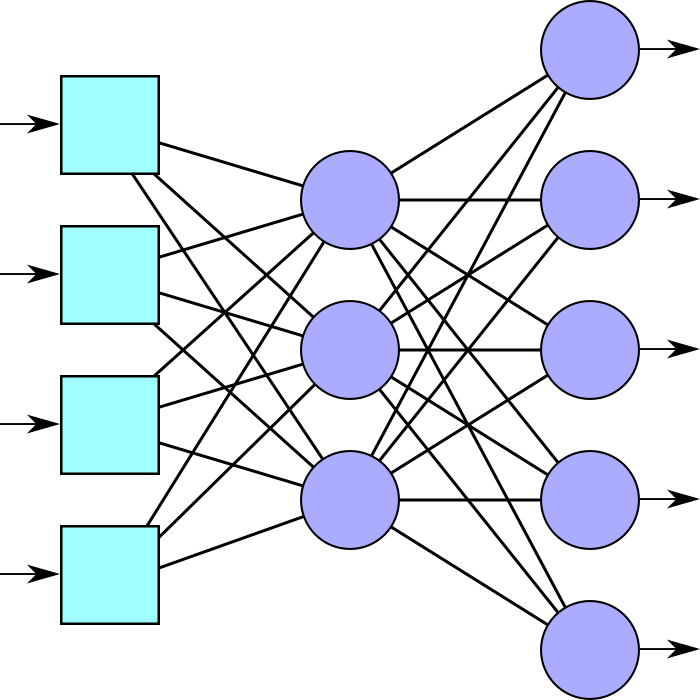
\includegraphics[width = 2.5in]{Figures/neural_net.png}
	\caption{Schematic of a feedforward ANN with a single hidden layer. The activation function is applied only to the hidden and output layers. The number of neurons depicted in each layer is meant to represent the \textit{relative} number used by the actual ANN.}
	\label{fig:ch4_neural_net}
\end{figure} 

POD modes and time-varying coefficients were computed from the velocity fields using the method of snapshots [Sirovich1987]; the kernel was defined as the two-component turbulent kinetic energy.
The instantaneous velocity fields were not preprocessed prior to the decomposition (that is, missing or spurious vectors were not replaced or interpolated).
As experimental noise in the velocity fields will be completely uncorrelated to the near-field measurements, it will be filtered out by the stochastic estimation and hence preprocessing is unnecessary.
Unlike many past researchers, the coefficients for every POD mode were estimated, rather than just the most energetic modes, for two reasons.
First, it is not guaranteed that an individual POD mode corresponds to a physically distinct turbulent flow structure or event - an event may be broken up into multiple POD modes of varying energy levels.
Secondly, the most energetic POD mode(s) is not necessarily the most relevant mode(s) for the acoustic generation process (see Jordan \etal [2007] for a modification to the standard POD kernel in order to mitigate this issue). 

Even though the network is estimating even the least-energetic modes, the current method is far more computationally efficient than directly estimating the velocity fields themselves.
By encoding spatial correlations in the POD expansion coefficients, estimation of the $N$ snapshots of $M \times K$ spatial locations has been reduced from a minimization problem of $N$ vectors of $2MK$ to one of $N$ vectors of $N$.
For the current experimental database, this means the system has been reduced from $290,508 \times 1500$ to $1500 \times 1500$.
The neural network now only needs to identify the temporal correlations between the pressure field and the individual POD coefficients; it does not need to learn the spatial correlations.

Learning was accomplished via the standard backpropagation method [Haykin1994], which approximates the error surface of the cost function using first-order derivatives; the error `propagates' backwards from the output neurons to the hidden neurons and the synaptic weights at each neuron are updated to identify the (hopefully, global) minimum of the cost function using gradient descent.
The cost function was defined as the mean-squared-error between the predicted and measured expansion coefficients for a given PIV image group.
The velocity field, $\mathbf{U}$ at a given instance, $k$, can be recovered from $N$ orthonormal modes, $\phi$, and time-varying expansion coefficients, $a_k$, as $\mathbf{U} = \sum_{n=0}^{N} a_{k}^{n} \phi^n$ \citep{Berkooz1993}.
The total energy of each mode is therefore encoded in $a_k^n$, which will serve as a simple energy weighting for the cost function (the importance of relative errors to the cost function will essentially be scaled by the energy in each particular mode).
Training of the network was performed using the roughly 1500 ensemble pressure-velocity blocks of data (a few PIV images in each set had to be discarded due to laser misfires); synaptic weights were updated base on the average of all blocks (batch processing) using a constant learning rate.
A well-known issue with the gradient descent optimization method is that it has a tendency to get trapped in local minima and fails to converge to the global minimum.
Therefore, sample results were also calculated using a much different learning algorithm: adaptive particle swarm optimization.
Details will not be presented here however, as the results were found to not differ substantially from those produced by the backpropagation algorithm (while requiring significantly higher computational resources).

\subsection{Reduced-Order Representation of the Flow-Field}
Ultimately, due to limitations both in the methodology as well as in the ability of the microphones to sense fine-scale turbulent fluctuations, the estimated velocity field is going to represent a reduced-order model of the jet.
This can be easily observed in \fig{fig:ch4_SEPOD_filtering}, where the measured axial velocity field at an arbitrary instance in time has been plotted against the velocity field produced by the SE-POD estimation from the near-field pressure at the same instance in time.
For comparison purposes, a reduced-order reconstruction of the measured velocity field from the first 100 POD modes (but without estimating from the near-field pressure using SE) has also been included.
Note that here the output of the model produced by SE-POD is being compared against a known output that the system is meant to match; this is not an evaluation of the \textit{predictive} power of the model but of the \textit{representative} power.
\begin{figure}
	\centering
	\begin{subfigure}{0.75\textwidth}
		\centering
		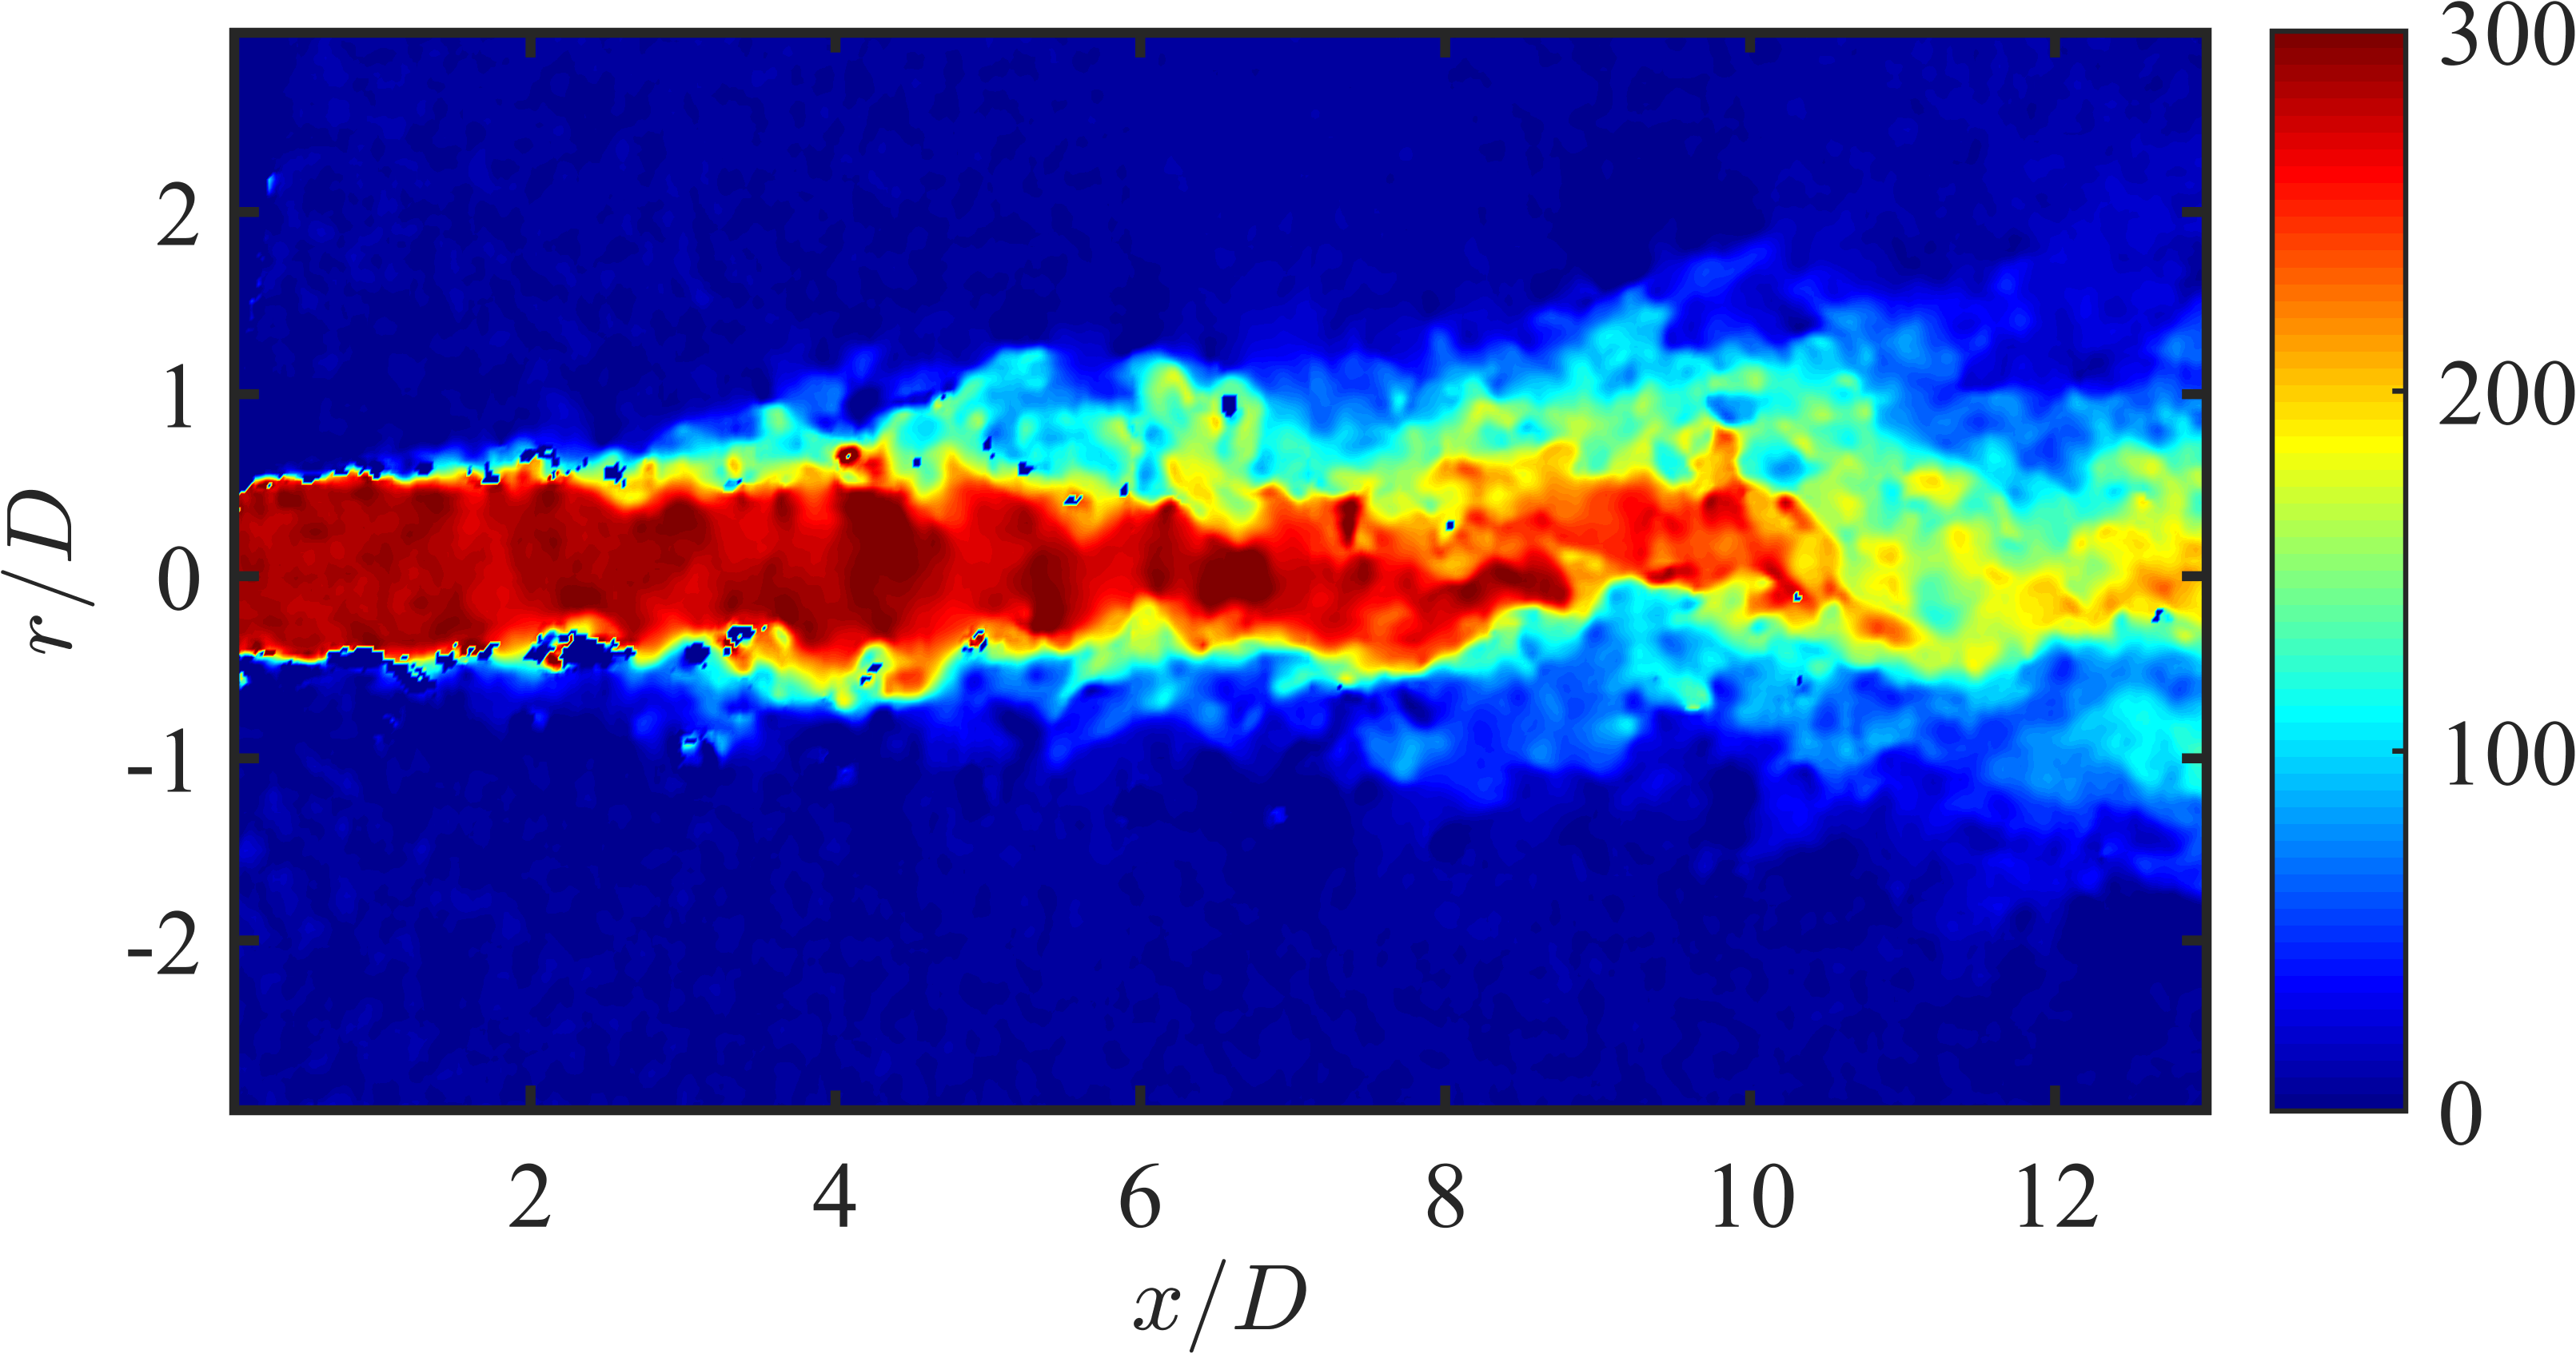
\includegraphics[width=0.95\linewidth]{Figures/ch4_Ux_true.png}
		\caption{Measured}
	\end{subfigure}\\
	\begin{subfigure}{0.75\textwidth}
		\centering
		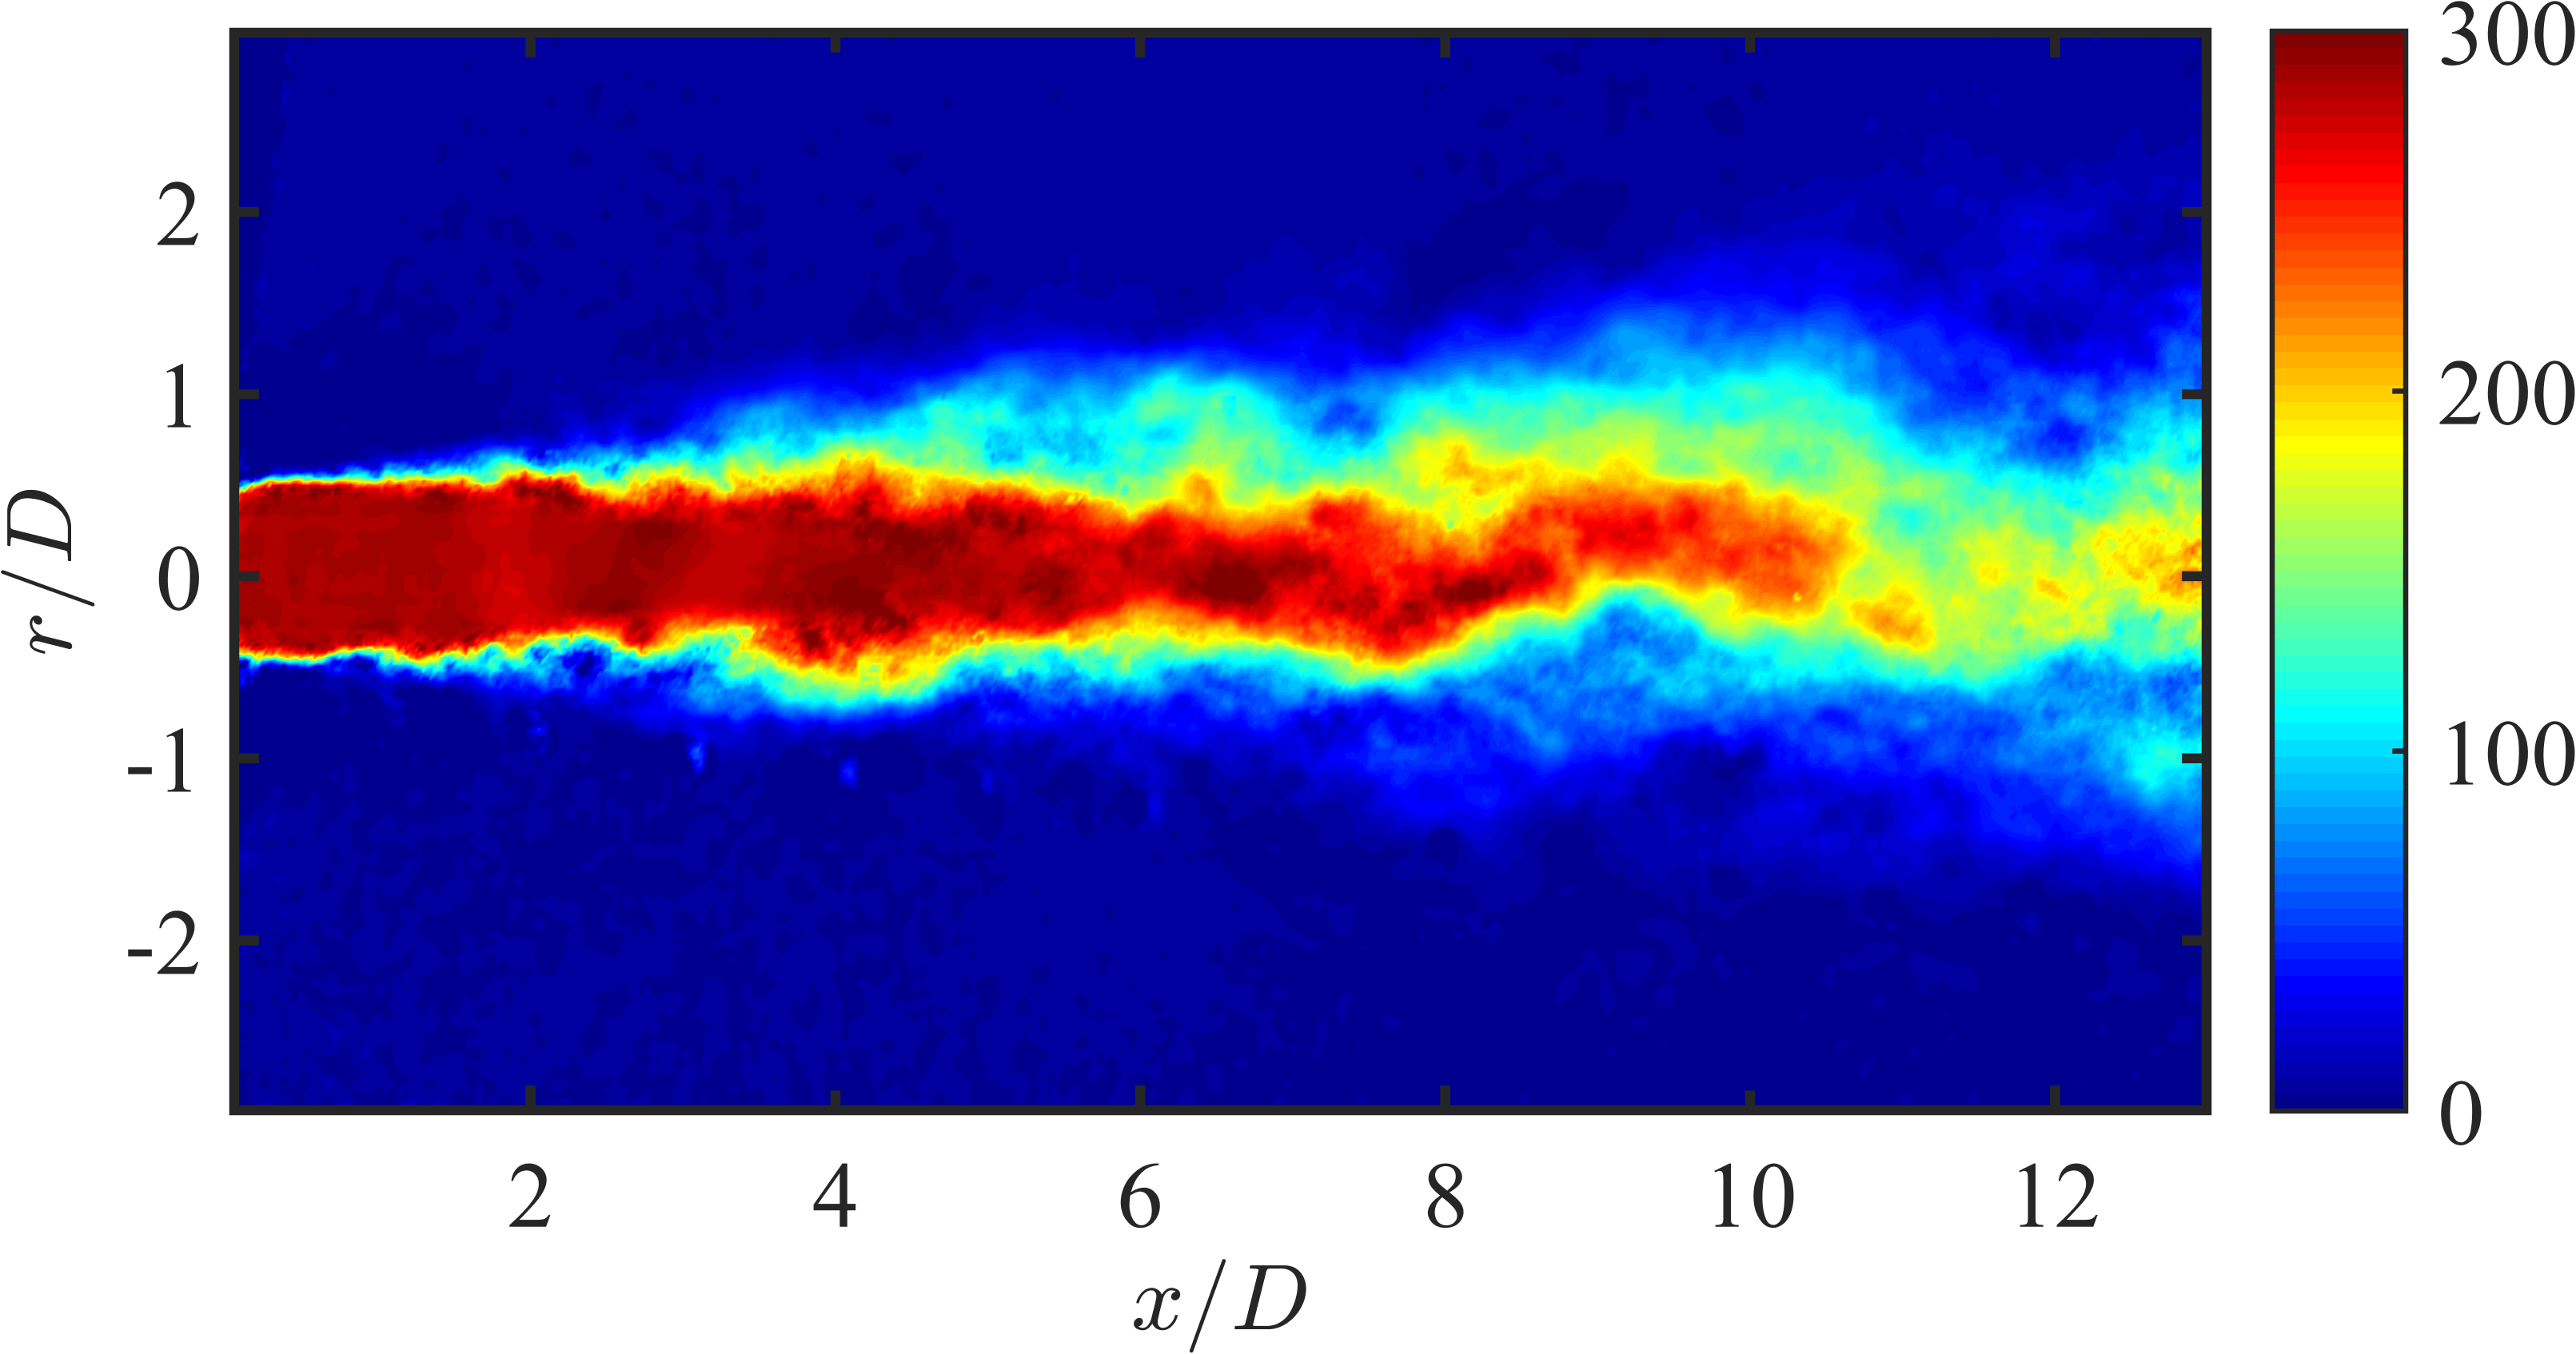
\includegraphics[width=0.95\linewidth]{Figures/ch4_Ux_estimated.png}
		\caption{Estimated}
	\end{subfigure}
	\begin{subfigure}{0.75\textwidth}
		\centering
		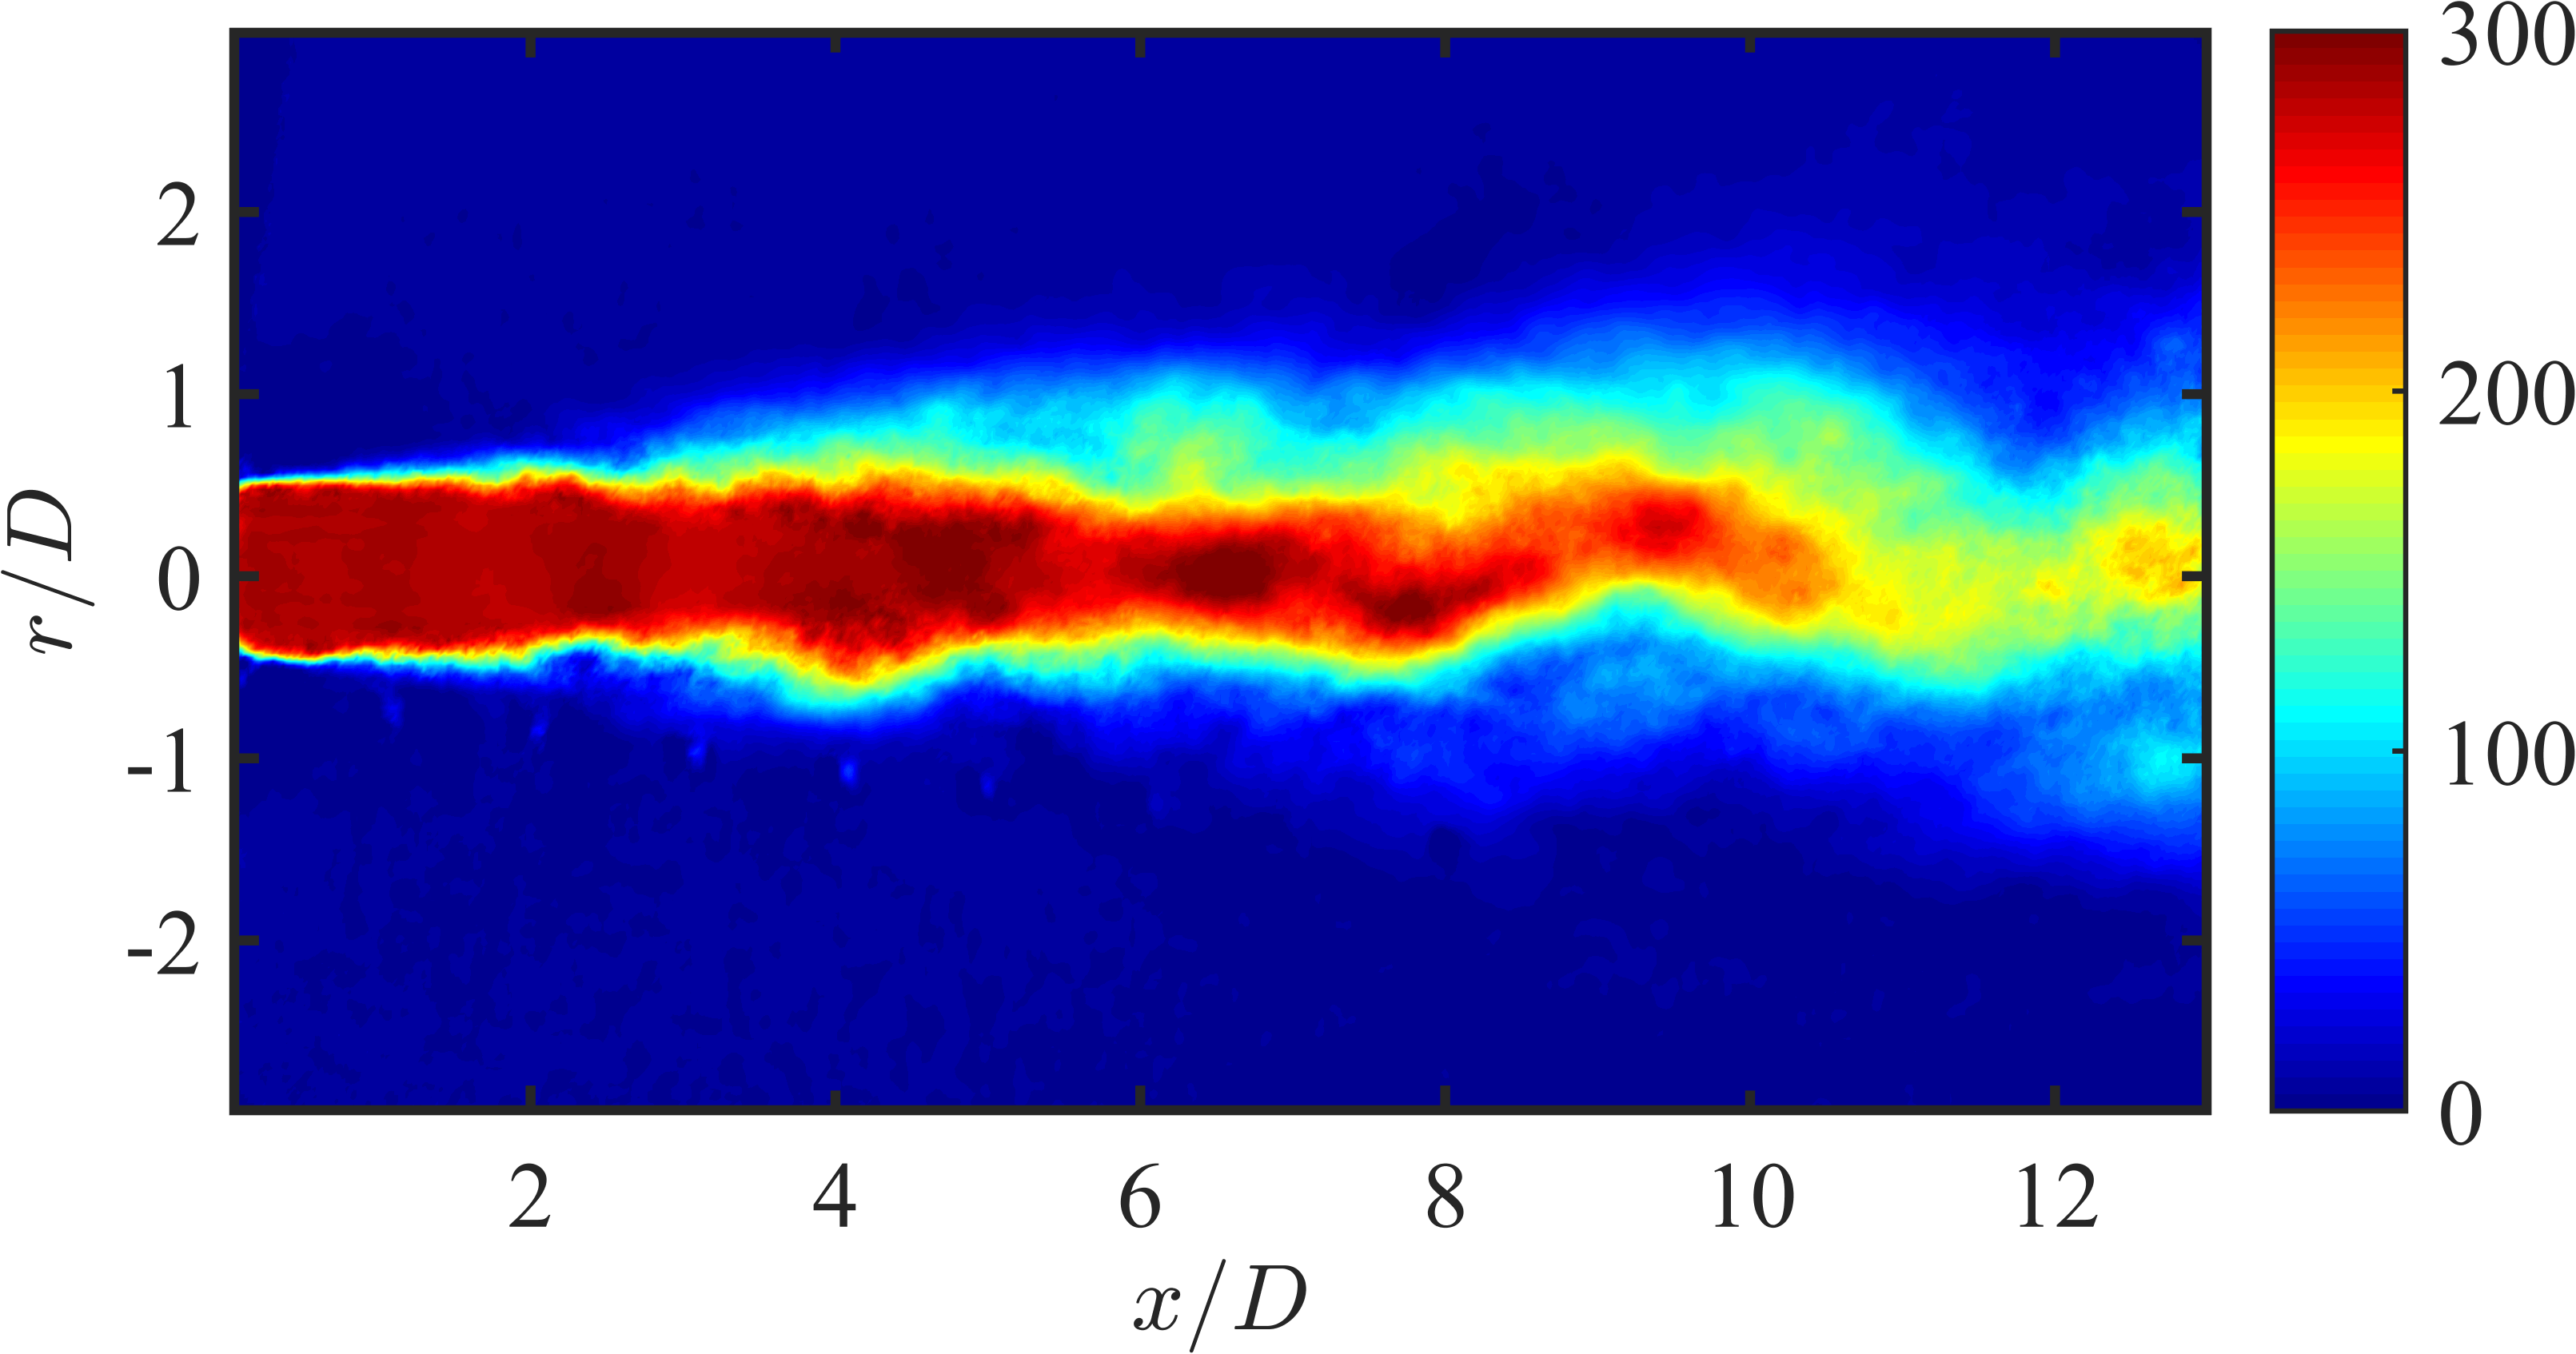
\includegraphics[width=0.95\linewidth]{Figures/ch4_Ux_POD100.png}
		\caption{First 100 POD modes}
	\end{subfigure}
	\caption{Comparison of a raw instantaneous axial velocity field $St_{DF} =0.05$ (a) against the same velocity field estimated from the near-field pressure (b) and finally a reduced-order reconstruction of the raw velocity using the first 100 POD modes ; units are in m/s.}
	\label{fig:ch4_SEPOD_filtering}
\end{figure}

As one would hope, the large-scale turbulent fluctuations are correctly identified by the SE-POD algorithm, and a mapping from the near-field pressure to this structures is appropriately generated.
The accuracy in the feature reproduction degrades considerably however as the scale of the turbulent eddy is reduced.
Some small-scale behavior is retained though most is filtered out, particularly the downstream region.
This was entirely expected however, as the reference signal is much more strongly damped with wavenumber than the conditional field being estimated (decay rates of $-20/3$ for the pressure field versus $-5/3$ for the velocity field).
The pressure field simply does not have the resolution to approximate the velocity field, particularly further downstream where the microphones are further from the jet centerline due to the spreading of the shear layer.
The estimated velocity fields are specifically referred to in the present work as \textit{reduced}-order rather than \textit{low}-order however.
Comparison of the estimated velocity against a reconstruction of the measured field using the most energetic 100 POD modes (of a total of 1500 POD modes corresponding to the 1500 uncorrelated velocity fields) indicates that the SE-POD algorithm is retain similar (if not greater) energy levels.
An example of this is the small-scale structure observed at $x/D \simeq 8$, just outside the high-velocity region of the jet (orange, in the figure in the measured velocity.
This distinct structure is still visible (though smeared and slightly reduced in amplitude) in the estimated velocity, though it is basically nonexistent in the 100-mode reconstruction which contains $\sim 50$\% of the fluctuating energy (see \fig{fig:ch4_modal_energy}).
While it is unlikely that this particular structure is notably important to the acoustic emission of the jet, low modal energy modulations of the large-scale structures may be.
Hence, it is desirable to retain as much of the information as possible when estimating the flow.

As a side note, the measured velocity fields retain some experimental errors from the PIV data processing; for instance, the small pockets of zero axial velocity observed on lower shear layer (particularly for $2 < x/D < 4$) in \fig{fig:ch4_SEPOD_filtering} are non-physical and correspond to missing vectors. 
As these experimental errors will be completely uncorrelated from the pressure signals, a conditional reconstruction will have great difficulty in reproducing them; in fact they \textit{should not} map from the pressure to the velocity at all.

It is also important to be mindful that an individual POD mode may not in fact correspond to anything physically distinct in the turbulent flow - it is after all, merely a mathematical construct which is based on no \textit{a priori} information of the system under investigation.
Tinney \etal [Tinney2008b] found that the modes produced by (spectral) POD had a tendency to appear in coupled pairs, and similar behavior is observed herein. 
For reference, the ten most energetic POD modes are shown in \fig{fig:ch4_St005_PODmodes} for $St_{DF} = 0.05$ and \fig{fig:ch4_St025_PODmodes} for $St_{DF} = 0.25$.
The characteristic scales of the excitation induced structures are smaller than the actual excitation period, as a result a significant amount of dead time occurs between LAFPA pulses during which the flow returns to its unperturbed state.
Because of this, analysis methods based on ensemble-averages of the velocity field show little difference between the baseline and $St_{DF} = 0.05$ excited jets (for this reason, the POD modes for the baseline jet are not shown).

For the impulsively-excited ($St_{DF} = 0.05$) jet, the dominant orthogonal modes are concentrated downstream of the end of the potential core, and it is not until mode 8 that a clear symmetric pattern about the jet centerline emerges. 
(However, it should be noted at modes 4 and 5 are very nearly mirrors of each other, and as such could produce symmetric features if coupled.)
Clearly, the excited axisymmetric structures represent only a small portion of the turbulent kinetic energy of the jet, and as such low-order representations of the flow will fail to accurately capture their dynamics.
As the excitation frequency is increased, the LAFPA-induced structures become high-energy periodic oscillations in the jet shear layer and core, and the POD modes are modified accordingly (\fig{fig:ch4_St025_PODmodes}).

Strong, axisymmetric fluctuations are now observed in the jet core for the first two POD modes, which match the wavelength of the excited structures (assuming $U_c \simeq 0.7 U_j$, per the two-point near-field correlations of Crawley \etal \citep{Crawley2015}) and which peak in amplitude near the end of the potential core.
The structure of mode 2 is quite similar to that of mode 1, differing only by a phase shift of $\pi/2$. 
This is a numerical artifact produced by the downstream convection of the large-scale structures (remember that while multiple time-delays have been incorporated into the stochastic estimation algorithm, the POD was computed using a single time-delay out of necessity).
Interestly, some of the higher modes, particularly mode 10, exhibit core fluctuations at a harmonic of the excitation wavelength.
As will be seen shortly, LAFPA excitation at this frequency yields higher-frequency structures which undergo a periodic merging to ultimately generate structures at the excitation frequency. 
These modes are capturing this process which might be highly relevant to the noise generation process. 
Lastly, even in the periodically-excited jet where the LAFPA-induced structures are the dominant POD modes, the modal energy convergence (\fig{fig:ch4_modal_energy}) of the POD modes is rather slow; as mentioned previously, 100 of the 1500 modes are required in order to capture 50\% of the total energy.
Again, this speaks to the necessity of accurately estimating not just the low-order modes, but the high-order as well.
\begin{figure}
	\centering
	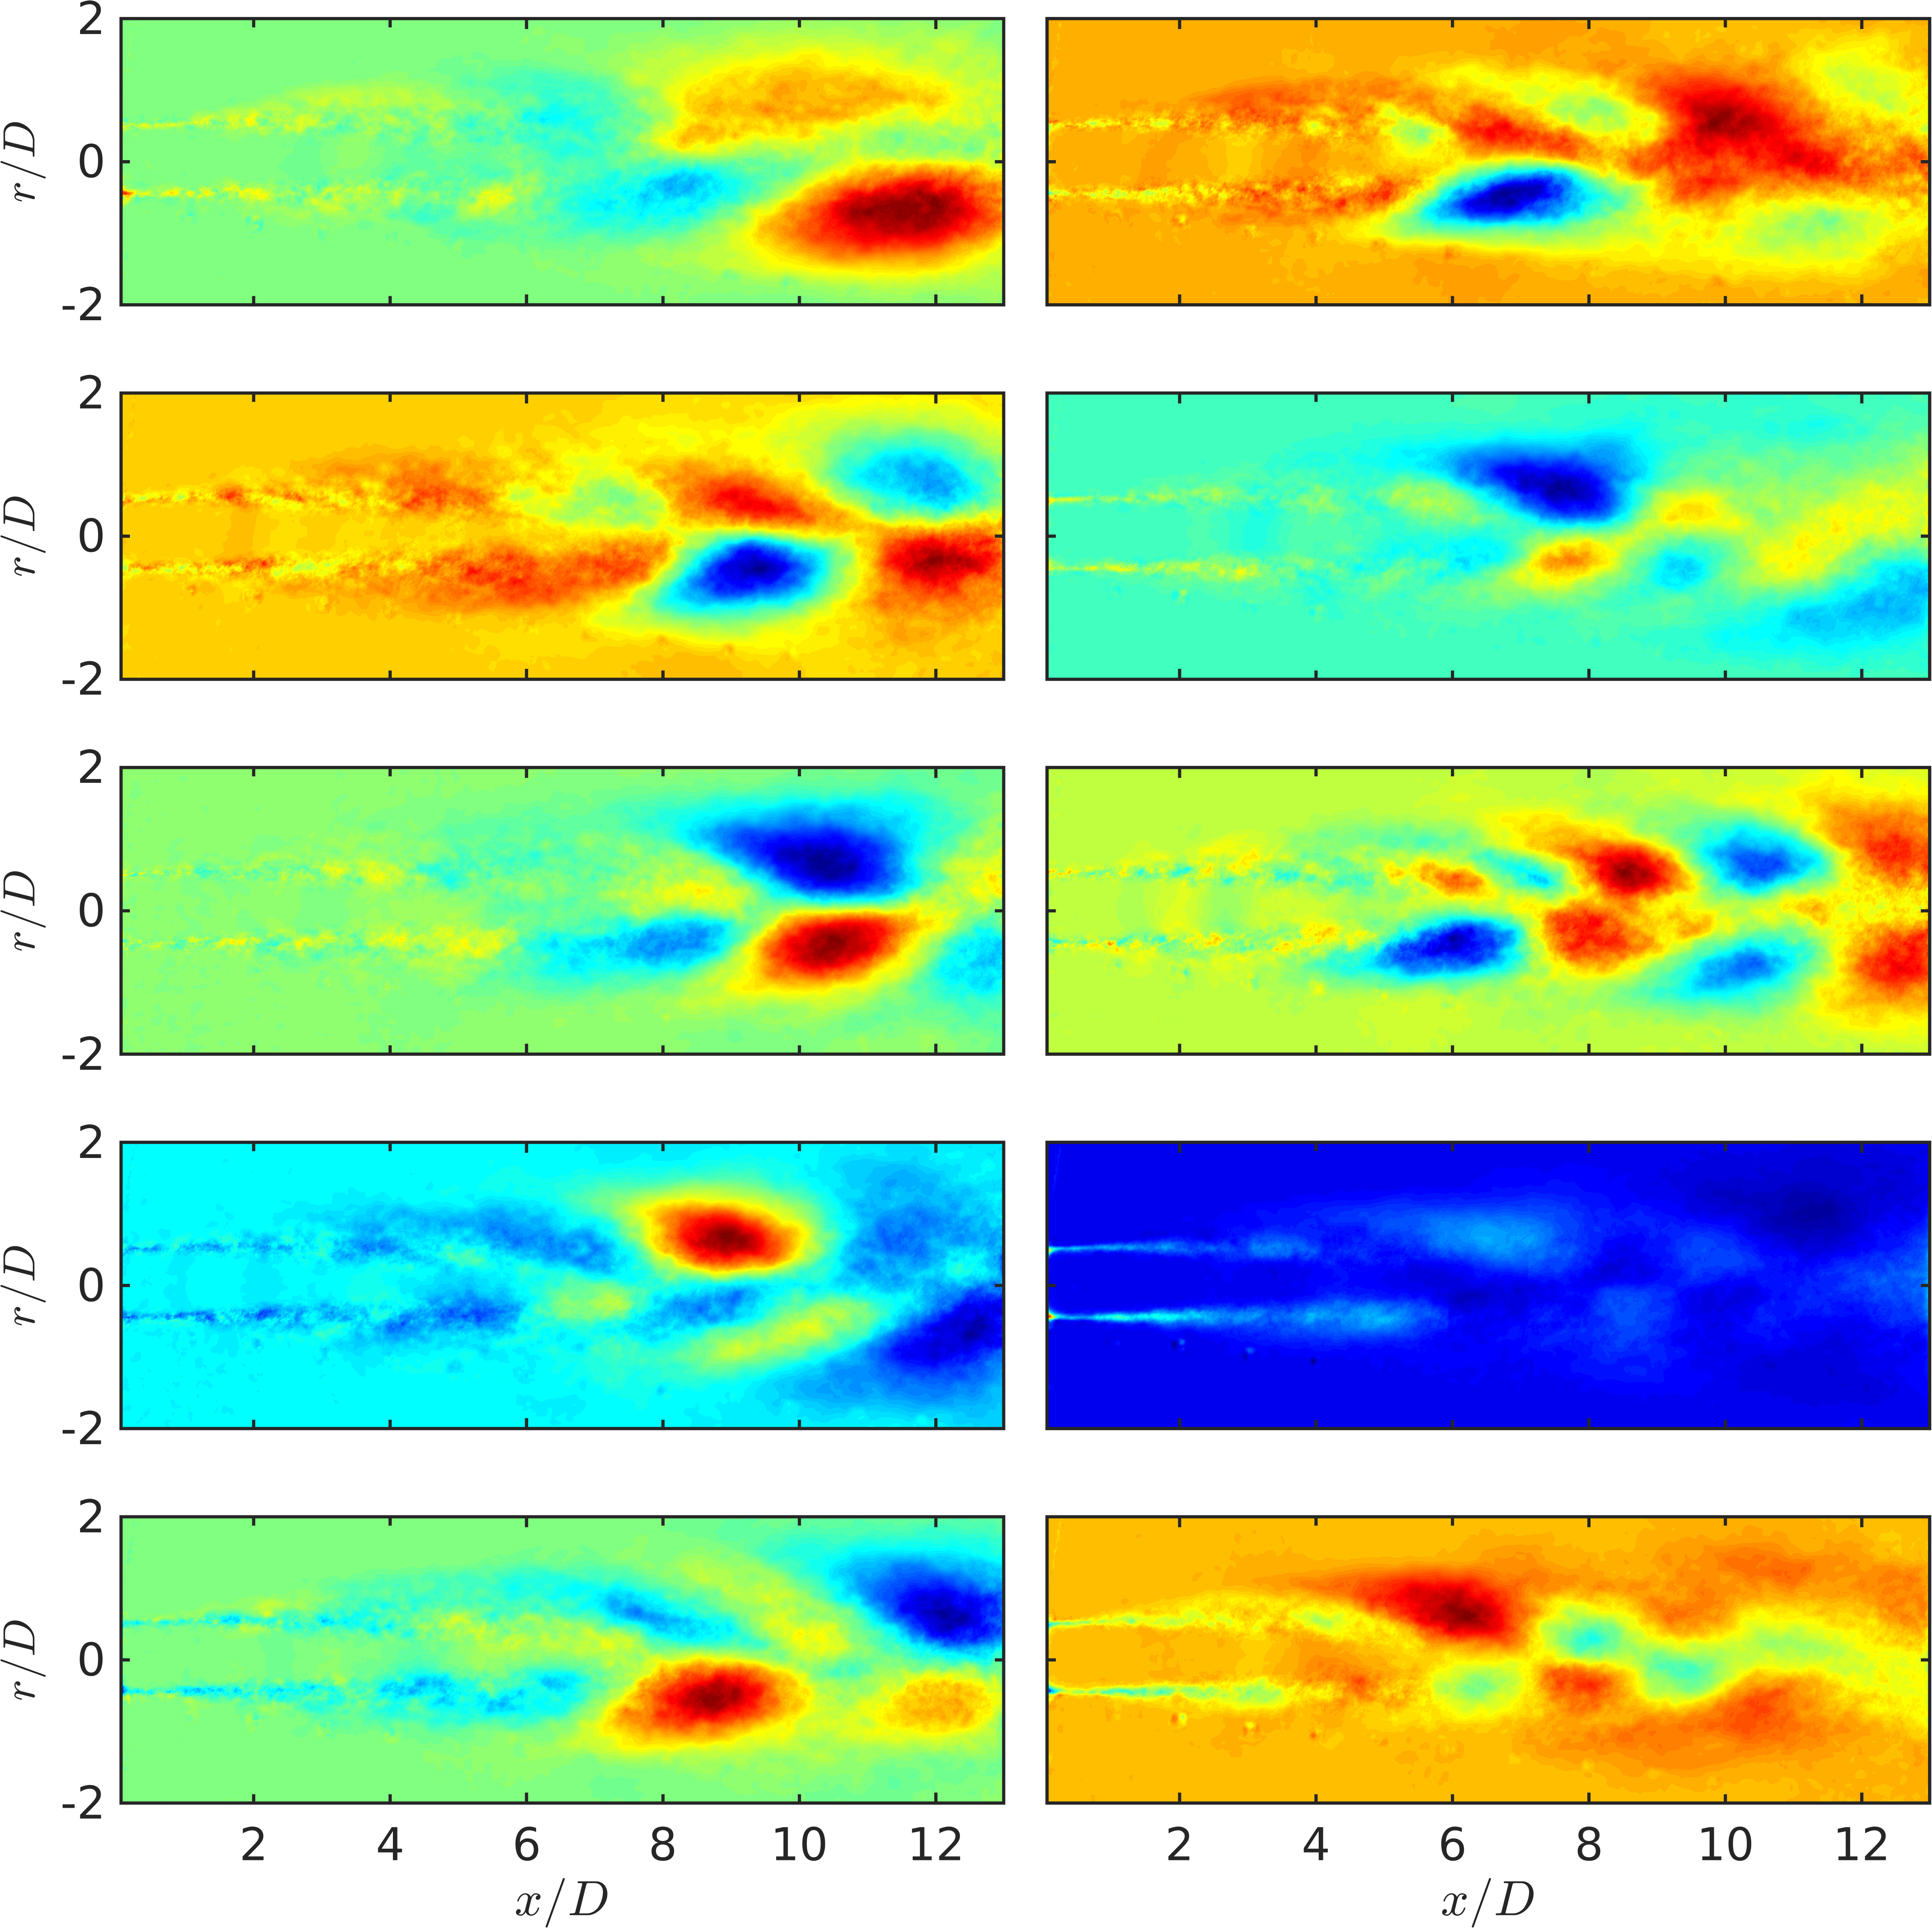
\includegraphics[width=1\linewidth]{Figures/ch4_St005_POD_Modes.png}
	\caption{First 10 POD modes (axial component only) for $St_{DF} = 0.05$, ordered top-down and then left-right.}
	\label{fig:ch4_St005_PODmodes}
\end{figure}
\begin{figure}
	\centering
	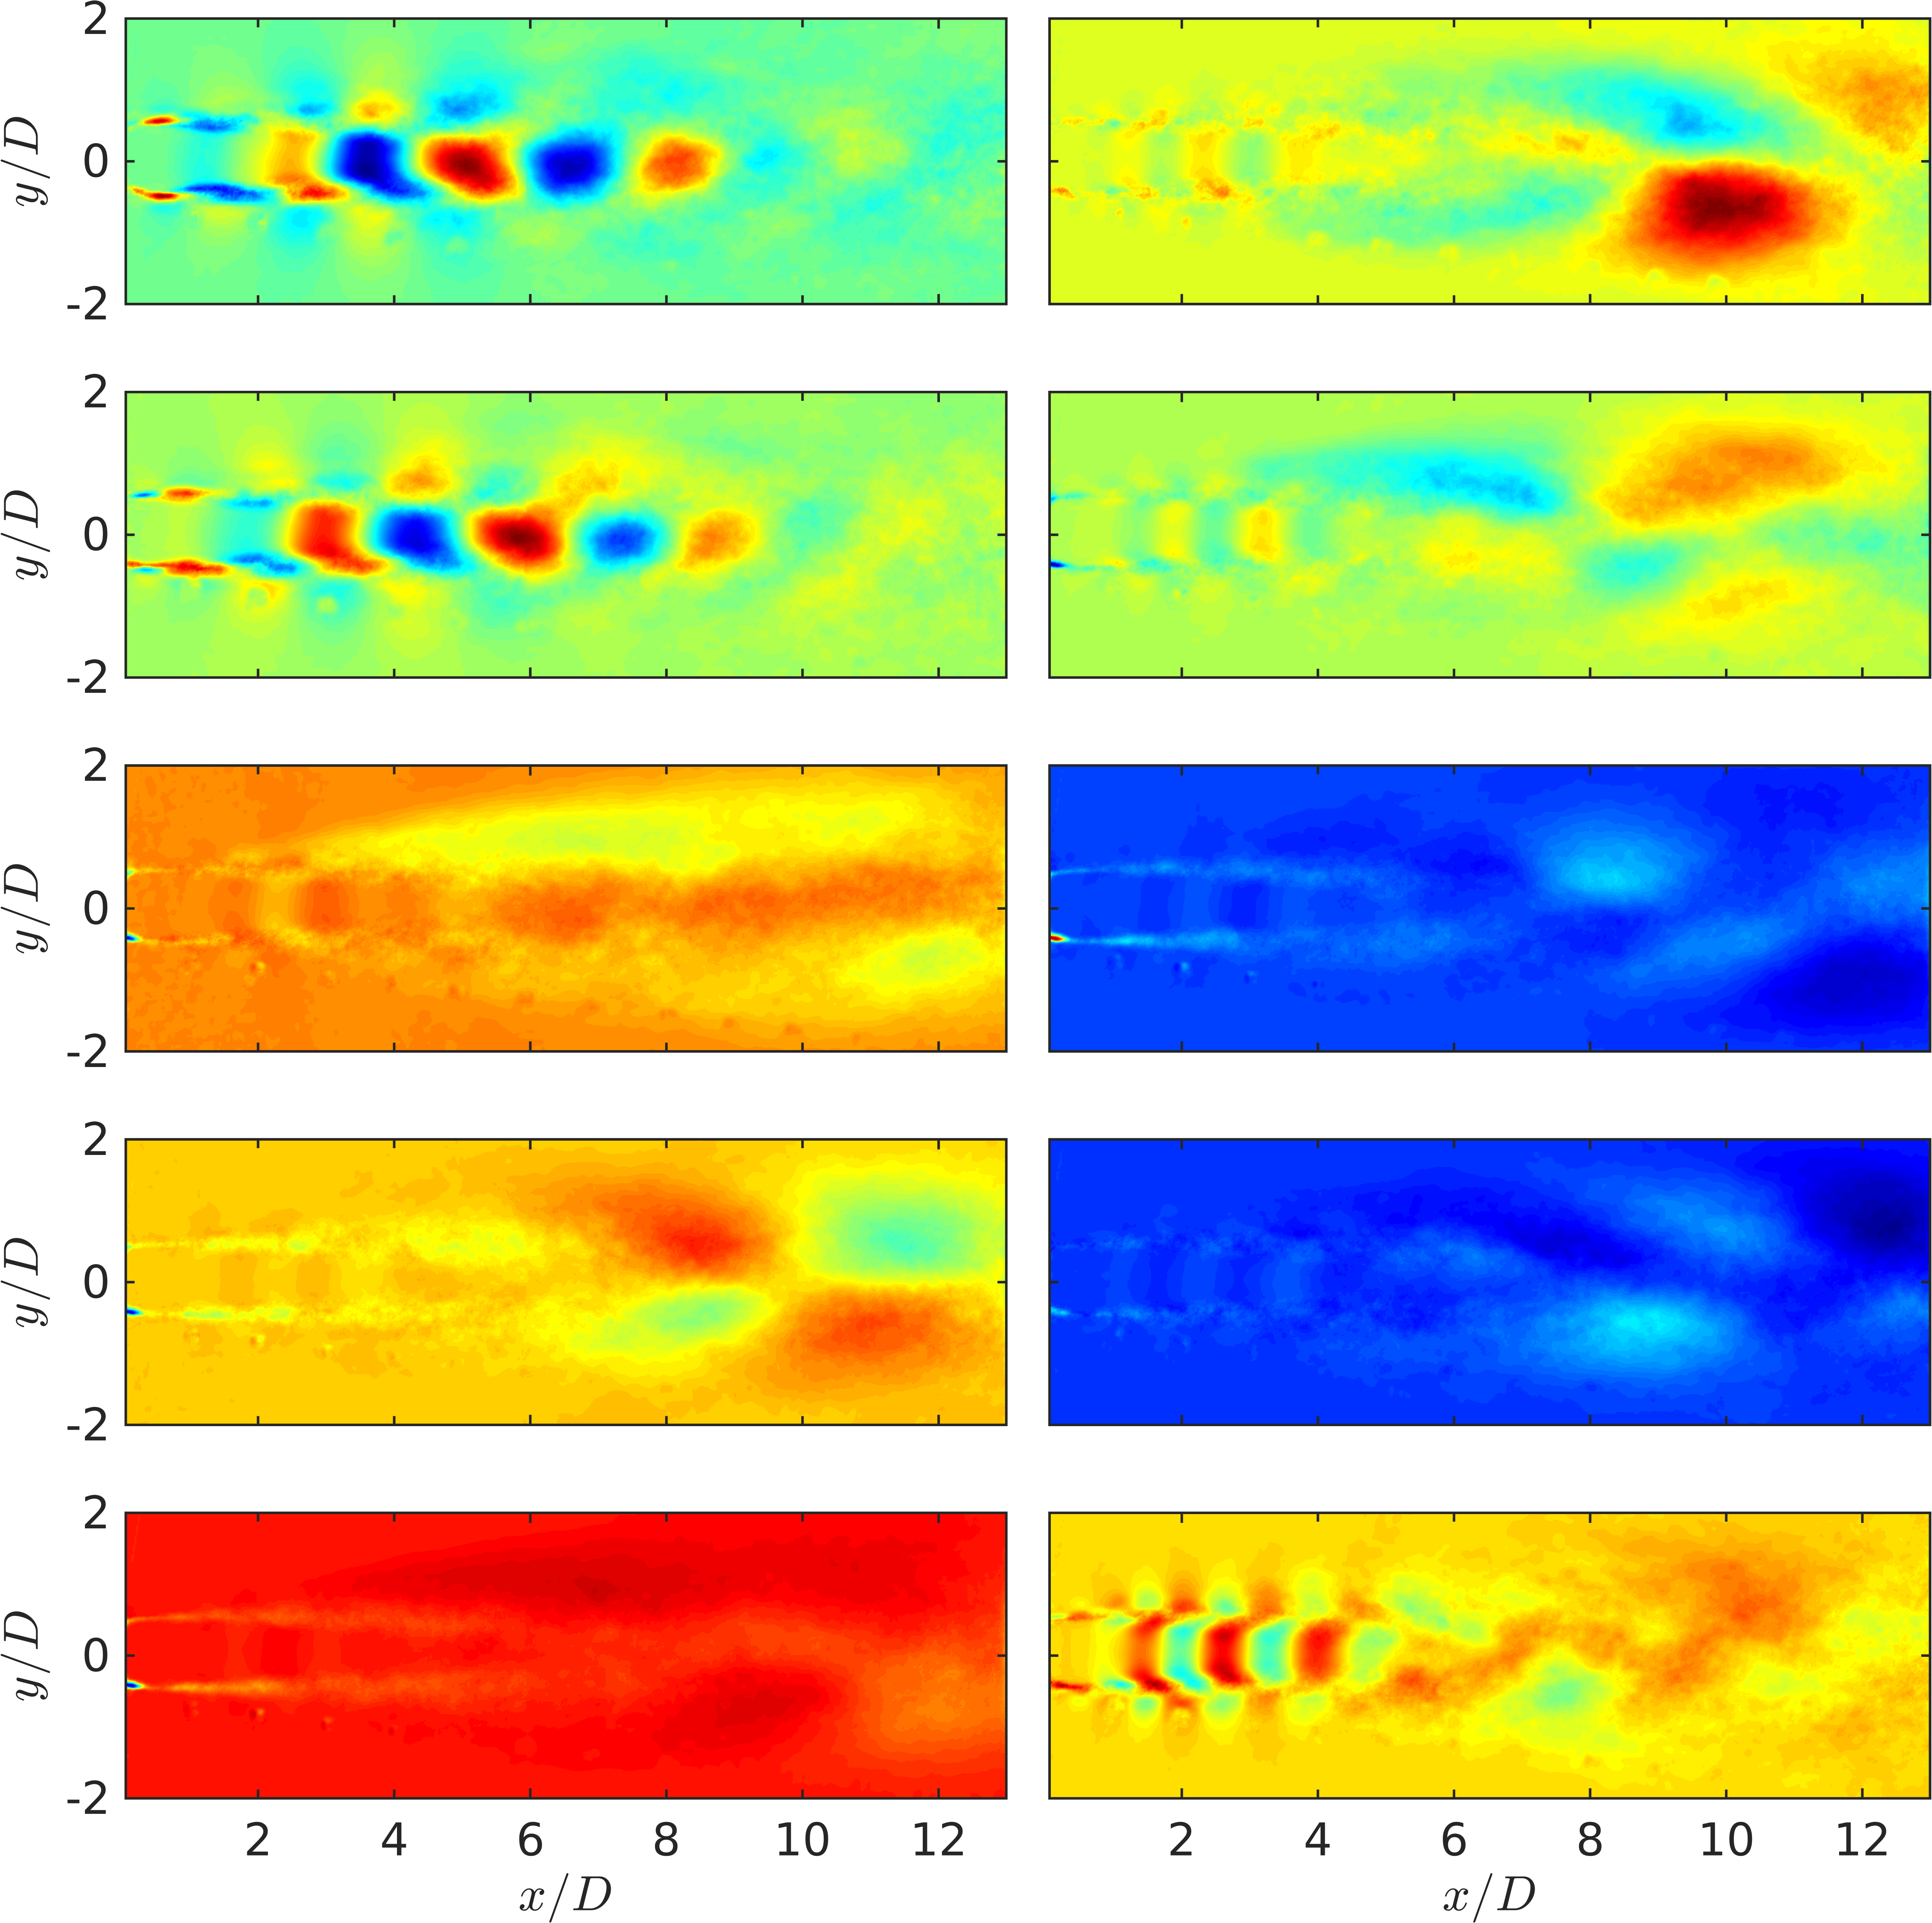
\includegraphics[width=1\linewidth]{Figures/ch4_St025_POD_Modes.png}
	\caption{First 10 POD modes (axial component only) for $St_{DF} = 0.25$, ordered top-down and then left-right.}
	\label{fig:ch4_St025_PODmodes}
\end{figure}
\begin{figure}
	\centering
	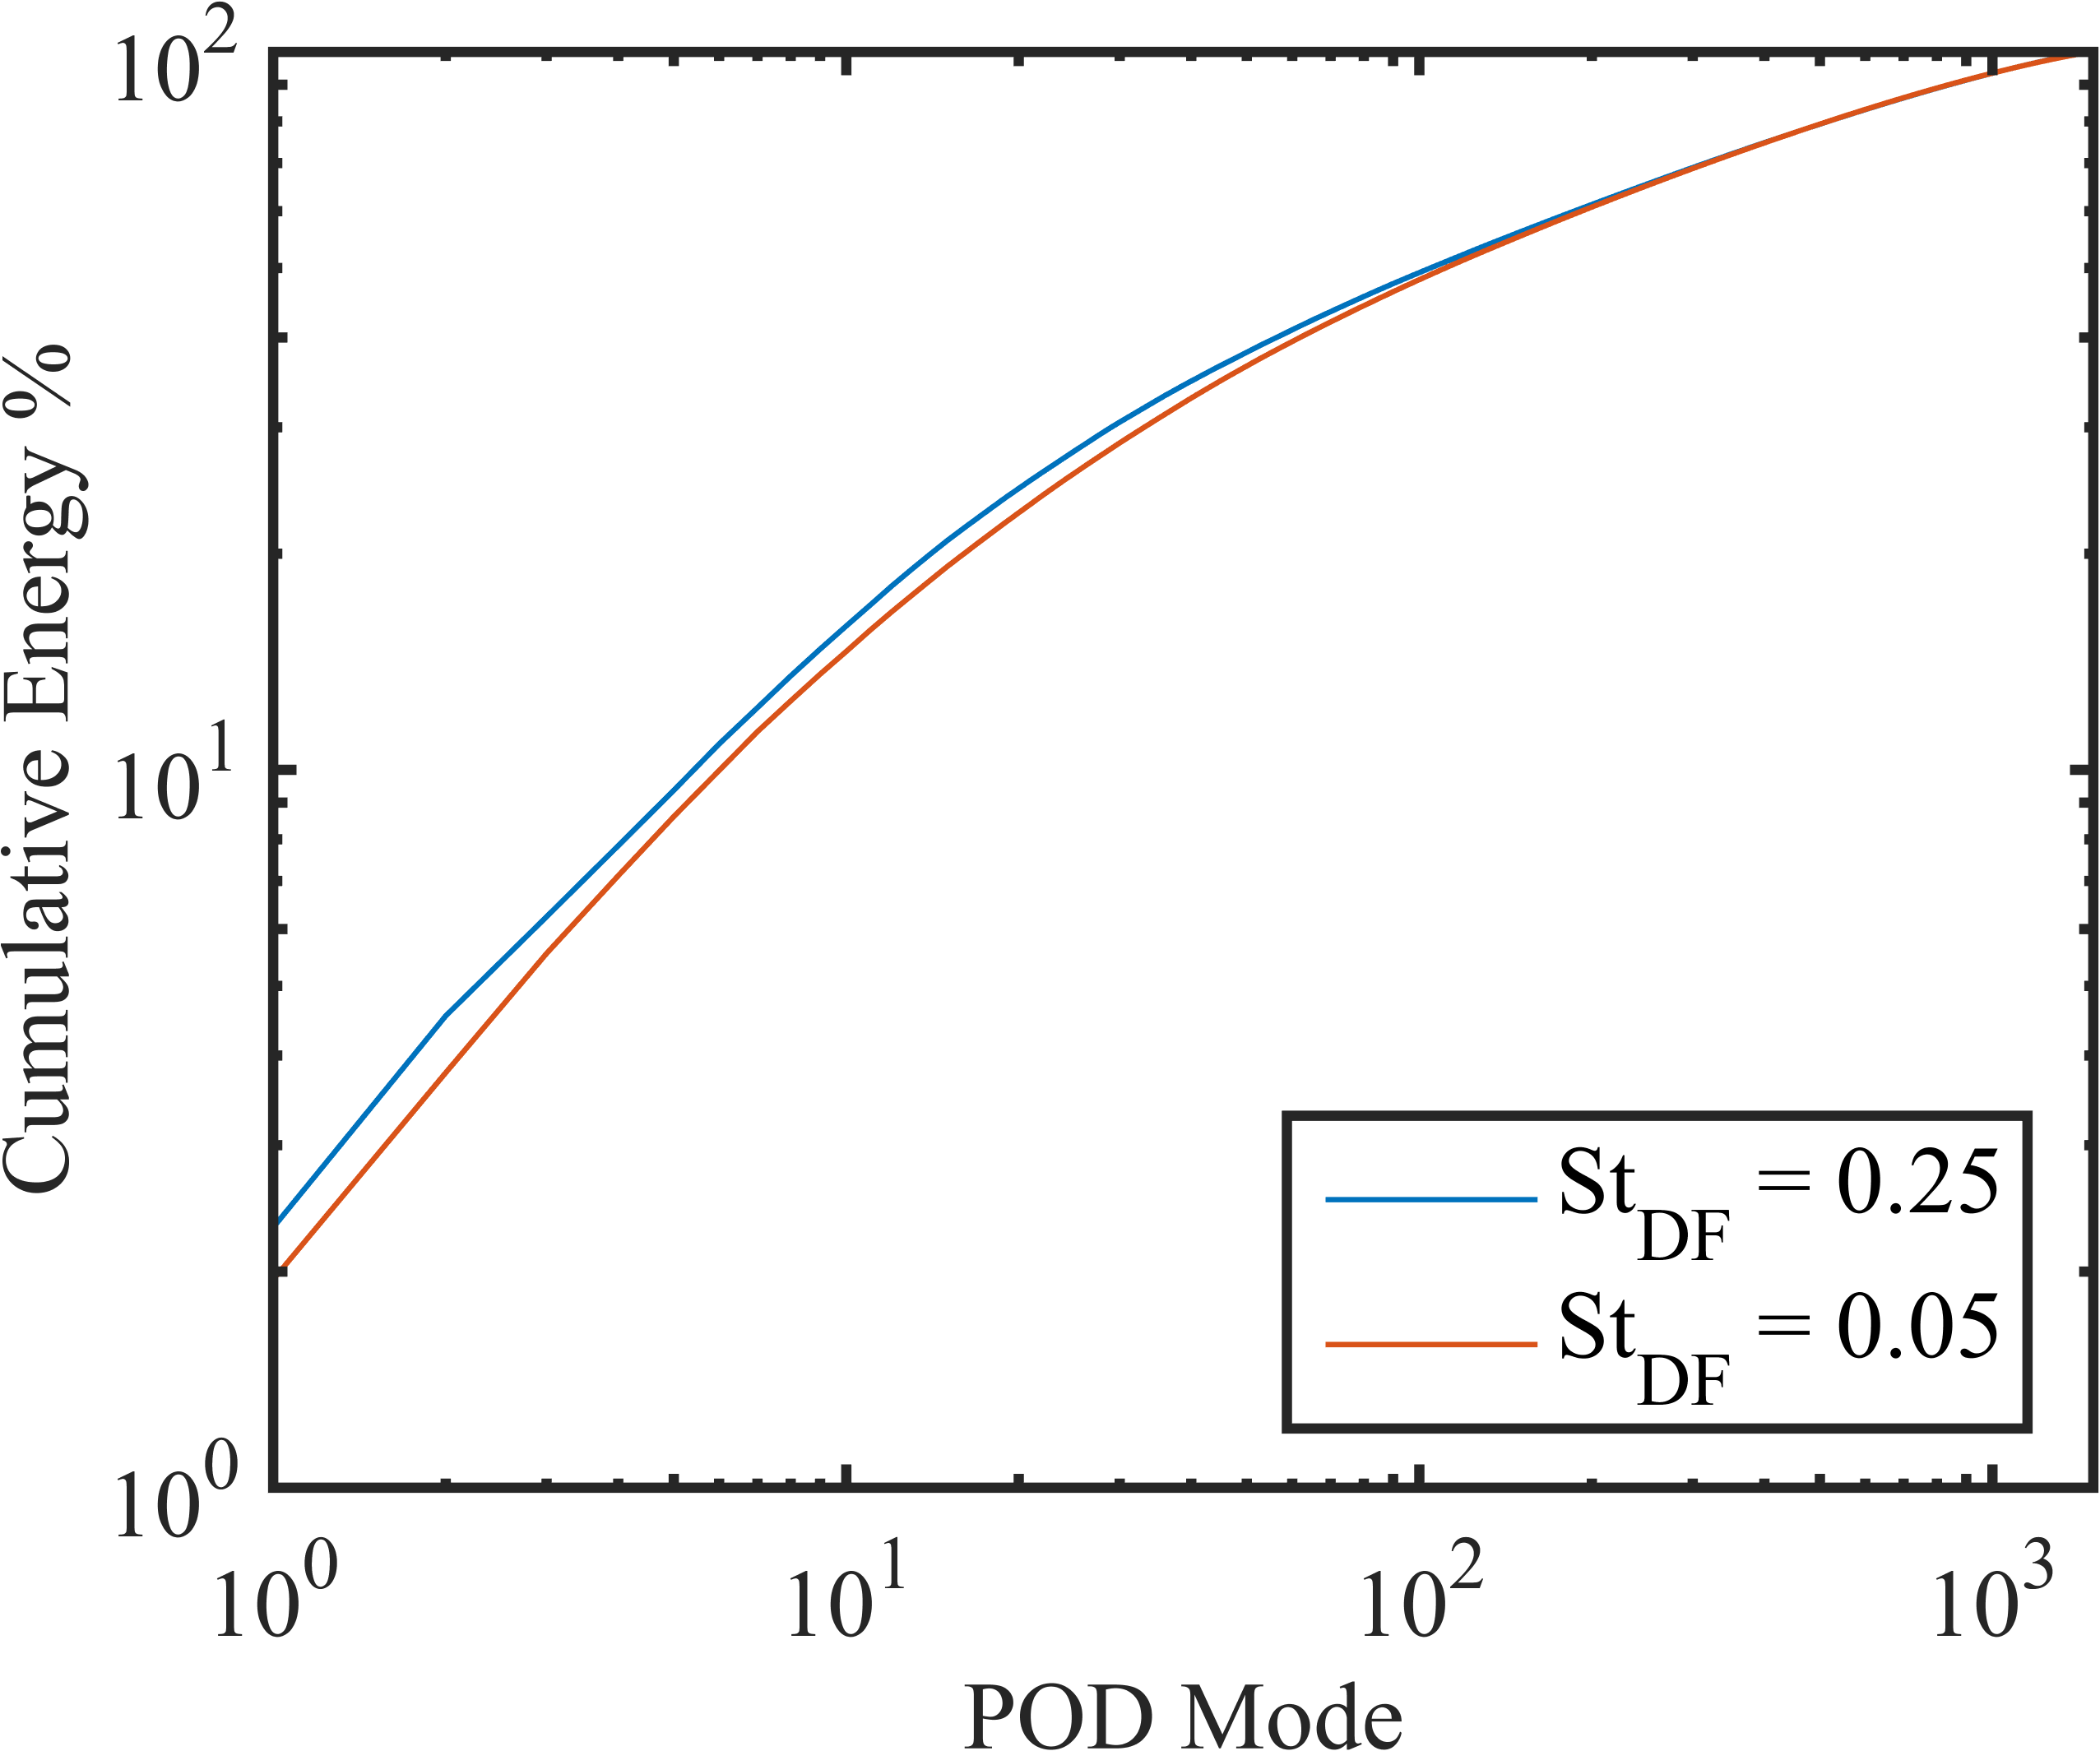
\includegraphics[width=3in]{Figures/ch4_POD_energies.png}
	\caption{POD modal energy convergence.}
	\label{fig:ch4_modal_energy}
\end{figure}


\section{Large-Scale Structure Interactions}
\subsection{Global Flow-Field Effects}
The global effects of excitation on shear layer development, both in general and in particular for LAFPAs, has been well-documented in the literature already (see Samimy \etal \citep{Samimy2012} for a review on LAFPA excitation in jets).
Therefore, only the features relevant to the current work will be briefly covered here.
Excitation produces highly-energetic structures which entrain the ambient fluid surrounding the shear layer, thus increasing mixing between the high-momentum core fluid and the ambient fluid.
As a result, the growth rate of the shear layer can be amplified significantly; this is illustrated in \fig{fig:ch4_shearlayerspreading}.
Excitation near the jet column mode ($St \simeq 0.35$) produces a rapid spreading of the initial shear layer until $x/D \simeq 5$, after which the spreading rate returns to the natural spreading rate.
(A quick note about the axial velocity fields shown in \fig{fig:ch4_shearlayerspreading}: the twelve circular regions of low velocity aligned on the outer edge of the lower shear layer are experimental artifacts. Laser reflections off of the microphones saturated the cameras, thus precluding the possibility of computing cross-correlations for these locations. Contrary to how it might appear in this figure, the microphone array is not in the flow-field, but situated behind from the cameras' point of view.)
\begin{figure}
	\centering
	\begin{subfigure}{0.75\textwidth}
		\centering
		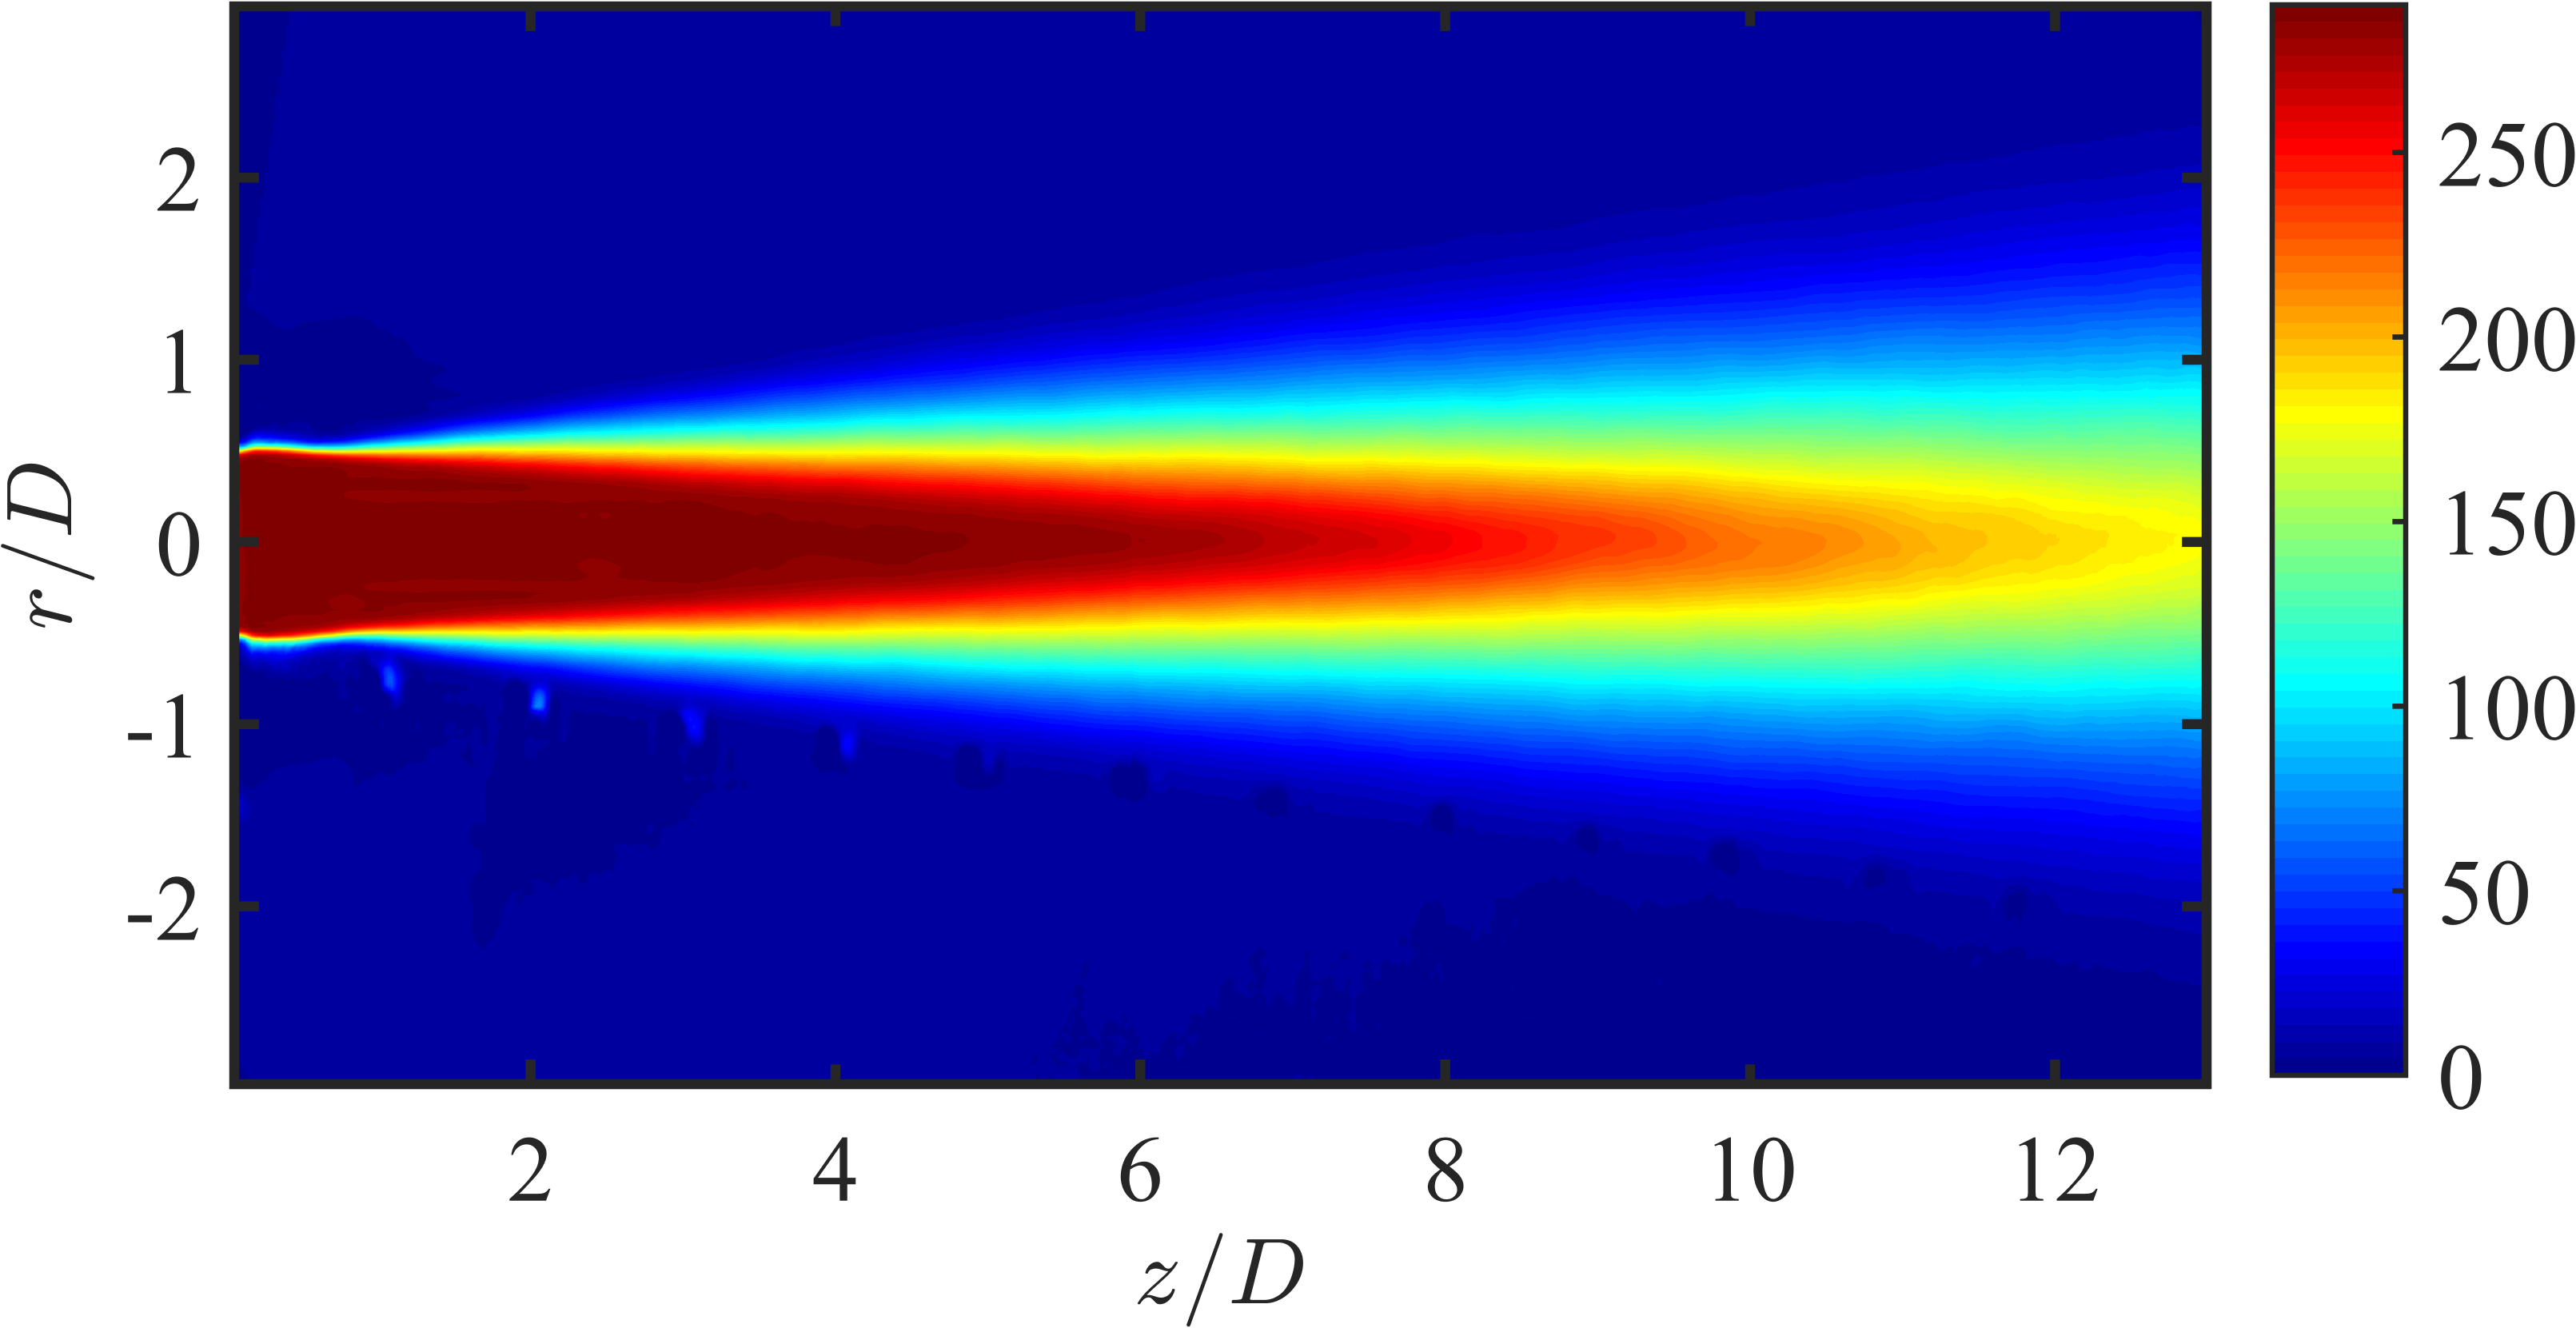
\includegraphics[width=0.95\linewidth]{Figures/ch4_St000_Um.png}
		\caption{Baseline}
	\end{subfigure}\\
	\begin{subfigure}{0.75\textwidth}
		\centering
		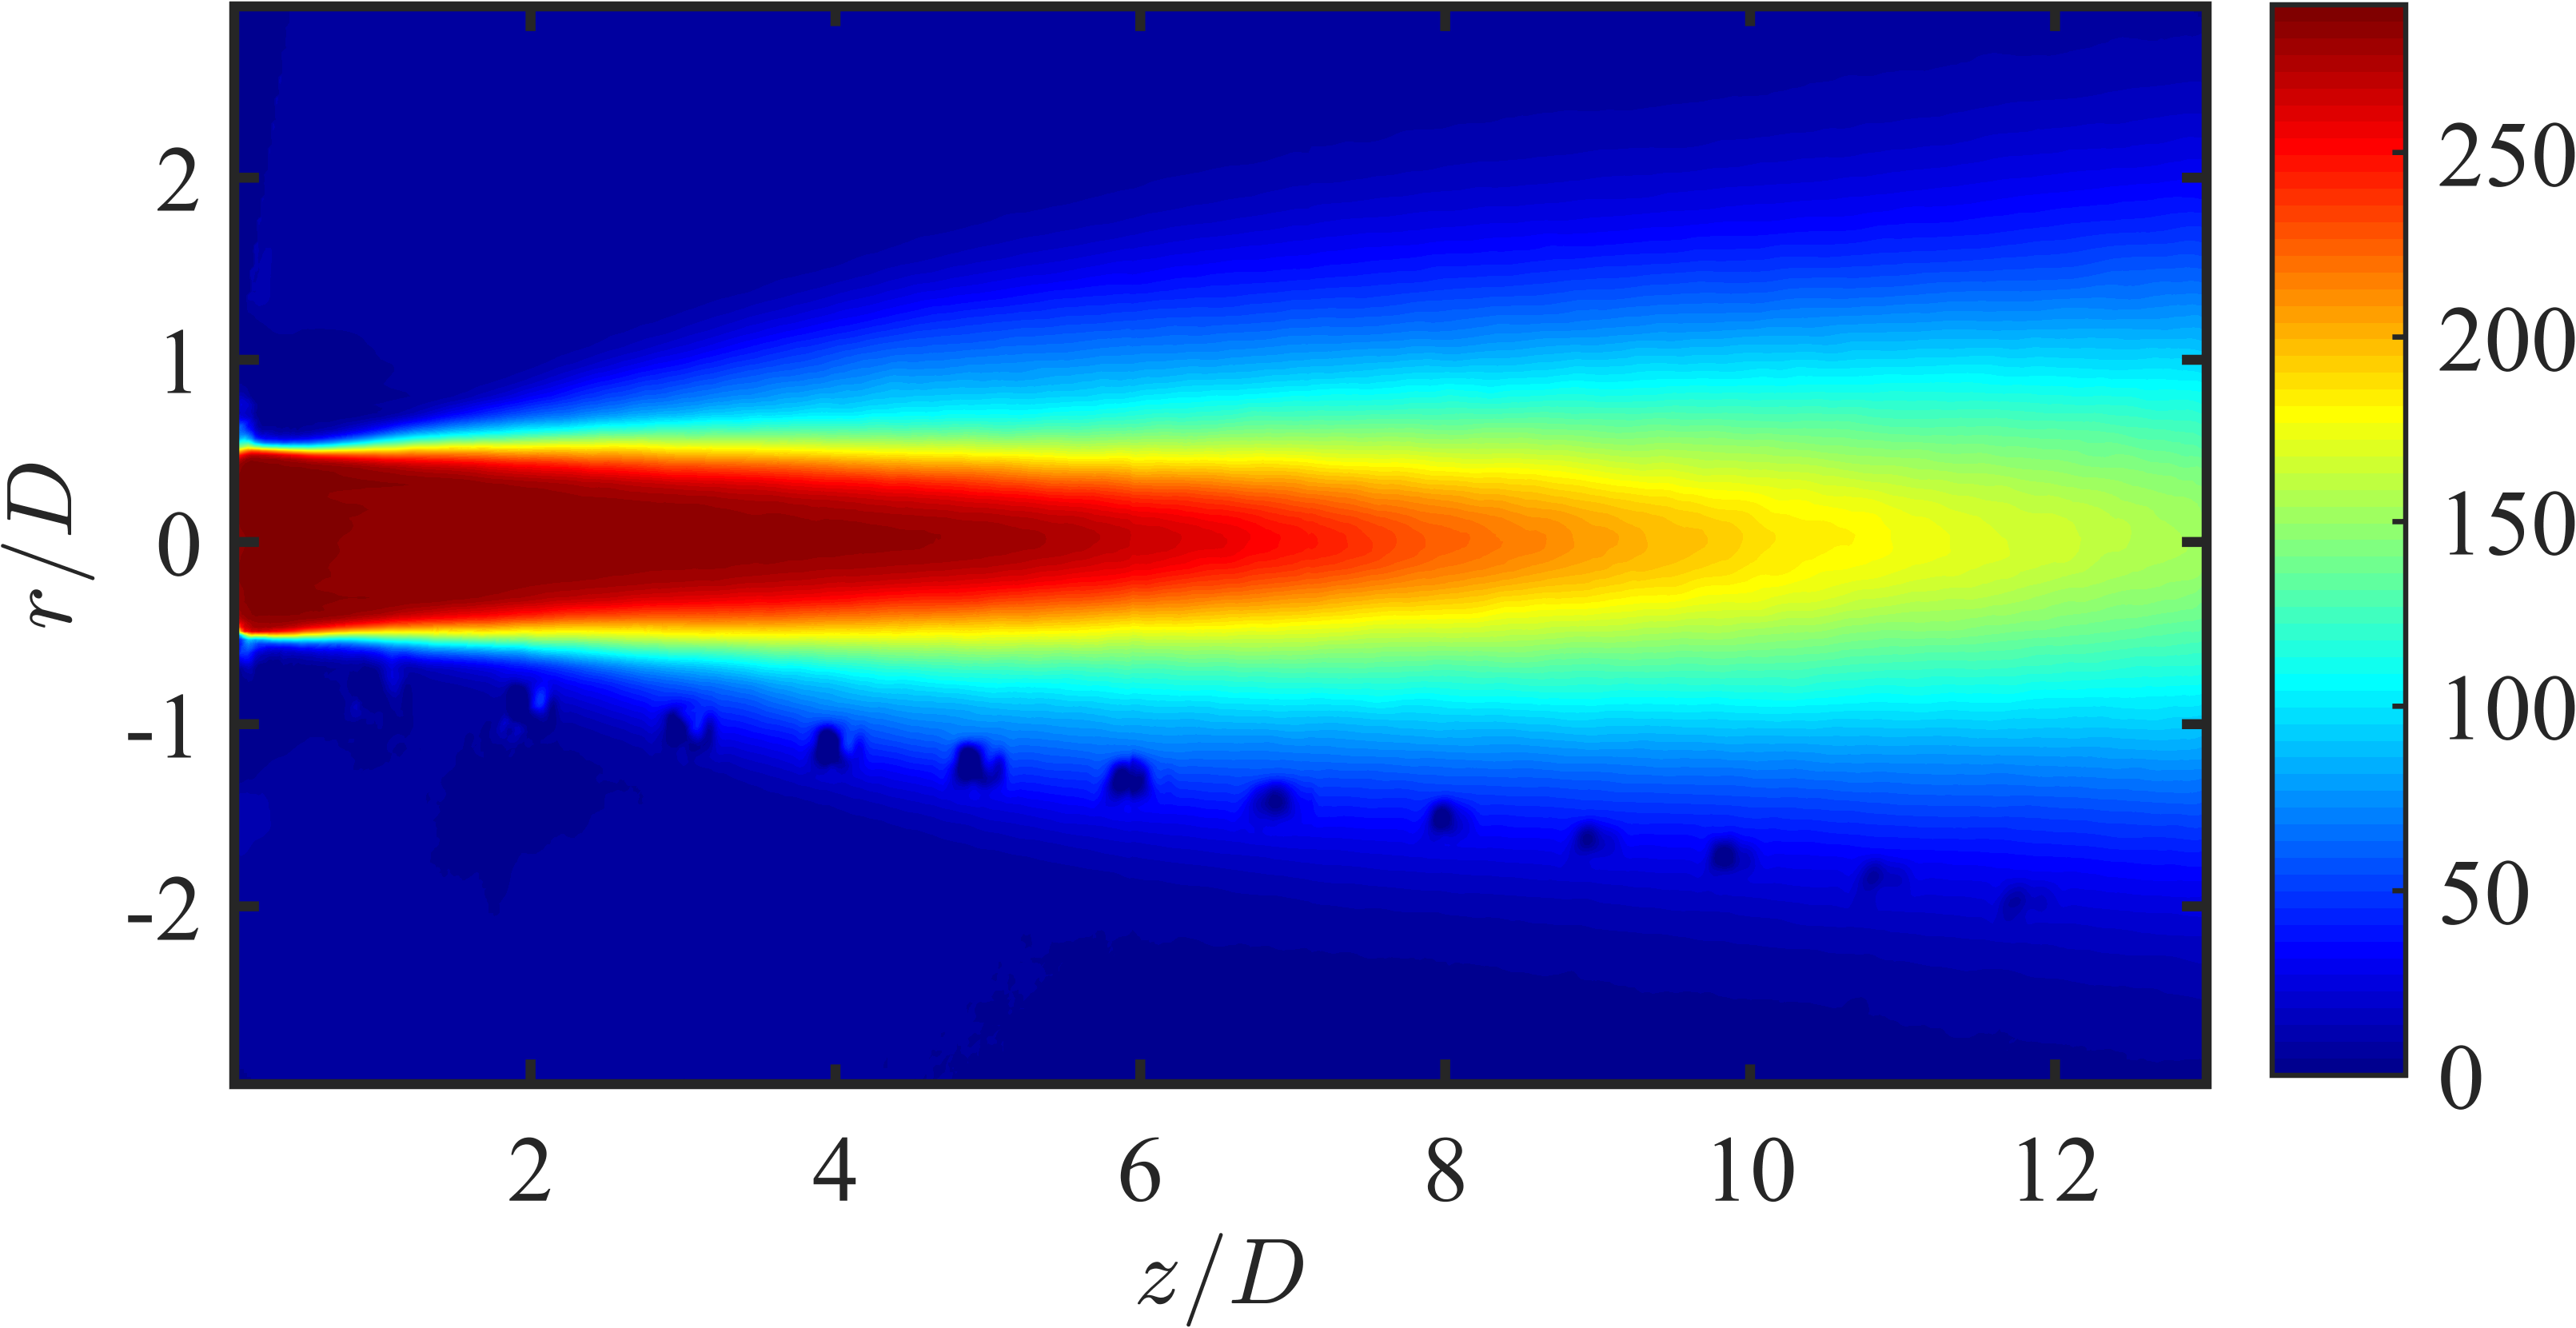
\includegraphics[width=0.95\linewidth]{Figures/ch4_St035_Um.png}
		\caption{$St_{DF} = 0.35$}
	\end{subfigure}
	\caption{Effect of excitation on the shear layer spreading rate, as visualized by the axial component of the velocity field.}
	\label{fig:ch4_shearlayerspreading}
\end{figure}

The increased mixing also affects the high-velocity side of the shear layer, resulting in a reduction in the length of the potential core.
In \fig{fig:ch4_centerlinemach}, the time-averaged centerline Mach number for each excitation case (as well as the natural jet) has been plotted as a function of axial distance.
A slow progression in the location of the end of the potential core is clearly evident, with it shifting upstream from $x/D \simeq 6$ eventually to $x/D \simeq 5$ as the excitation Strouhal number nears the jet preferred frequency of $St_{DF} \simeq 0.35$ (though not shown here, above this excitation frequency the effect is reduced).
The end of the potential core is of particular interest for the current work, as previous researchers have indicated that the dominant noise generation mechanism is associated with the violent breakdown of large-scale axisymmetric structures as they pass through this location \citep{Hileman2005}.
The two-point correlations of \sect{sect:nearfield}, which identified the dominant noise source region as occurring near the end of the potential core, hint at this as well.

The breakdown of the large-scale axisymmetric structures occurs because as the shear layers merge, the interface between the interior sides of the ring vortex becomes highly unstable, so any small perturbations quickly grow and destroy the vortex.
The exact location at which this breakdown occurs is ultimately going to be a function of structure growth rate, as larger structures will self-interact further upstream.
The location of the end of the potential core is therefore dependent on the passage of the large-scale structures, and hence is not strictly constant in time [who to cite here?].
Therefore, an axial shift in the time-averaged acoustic source is not necessarily reflective of a changing source mechanism, but may instead simply indicate that the source mechanism is now occurring at a different location.
\begin{figure}
	\centering
	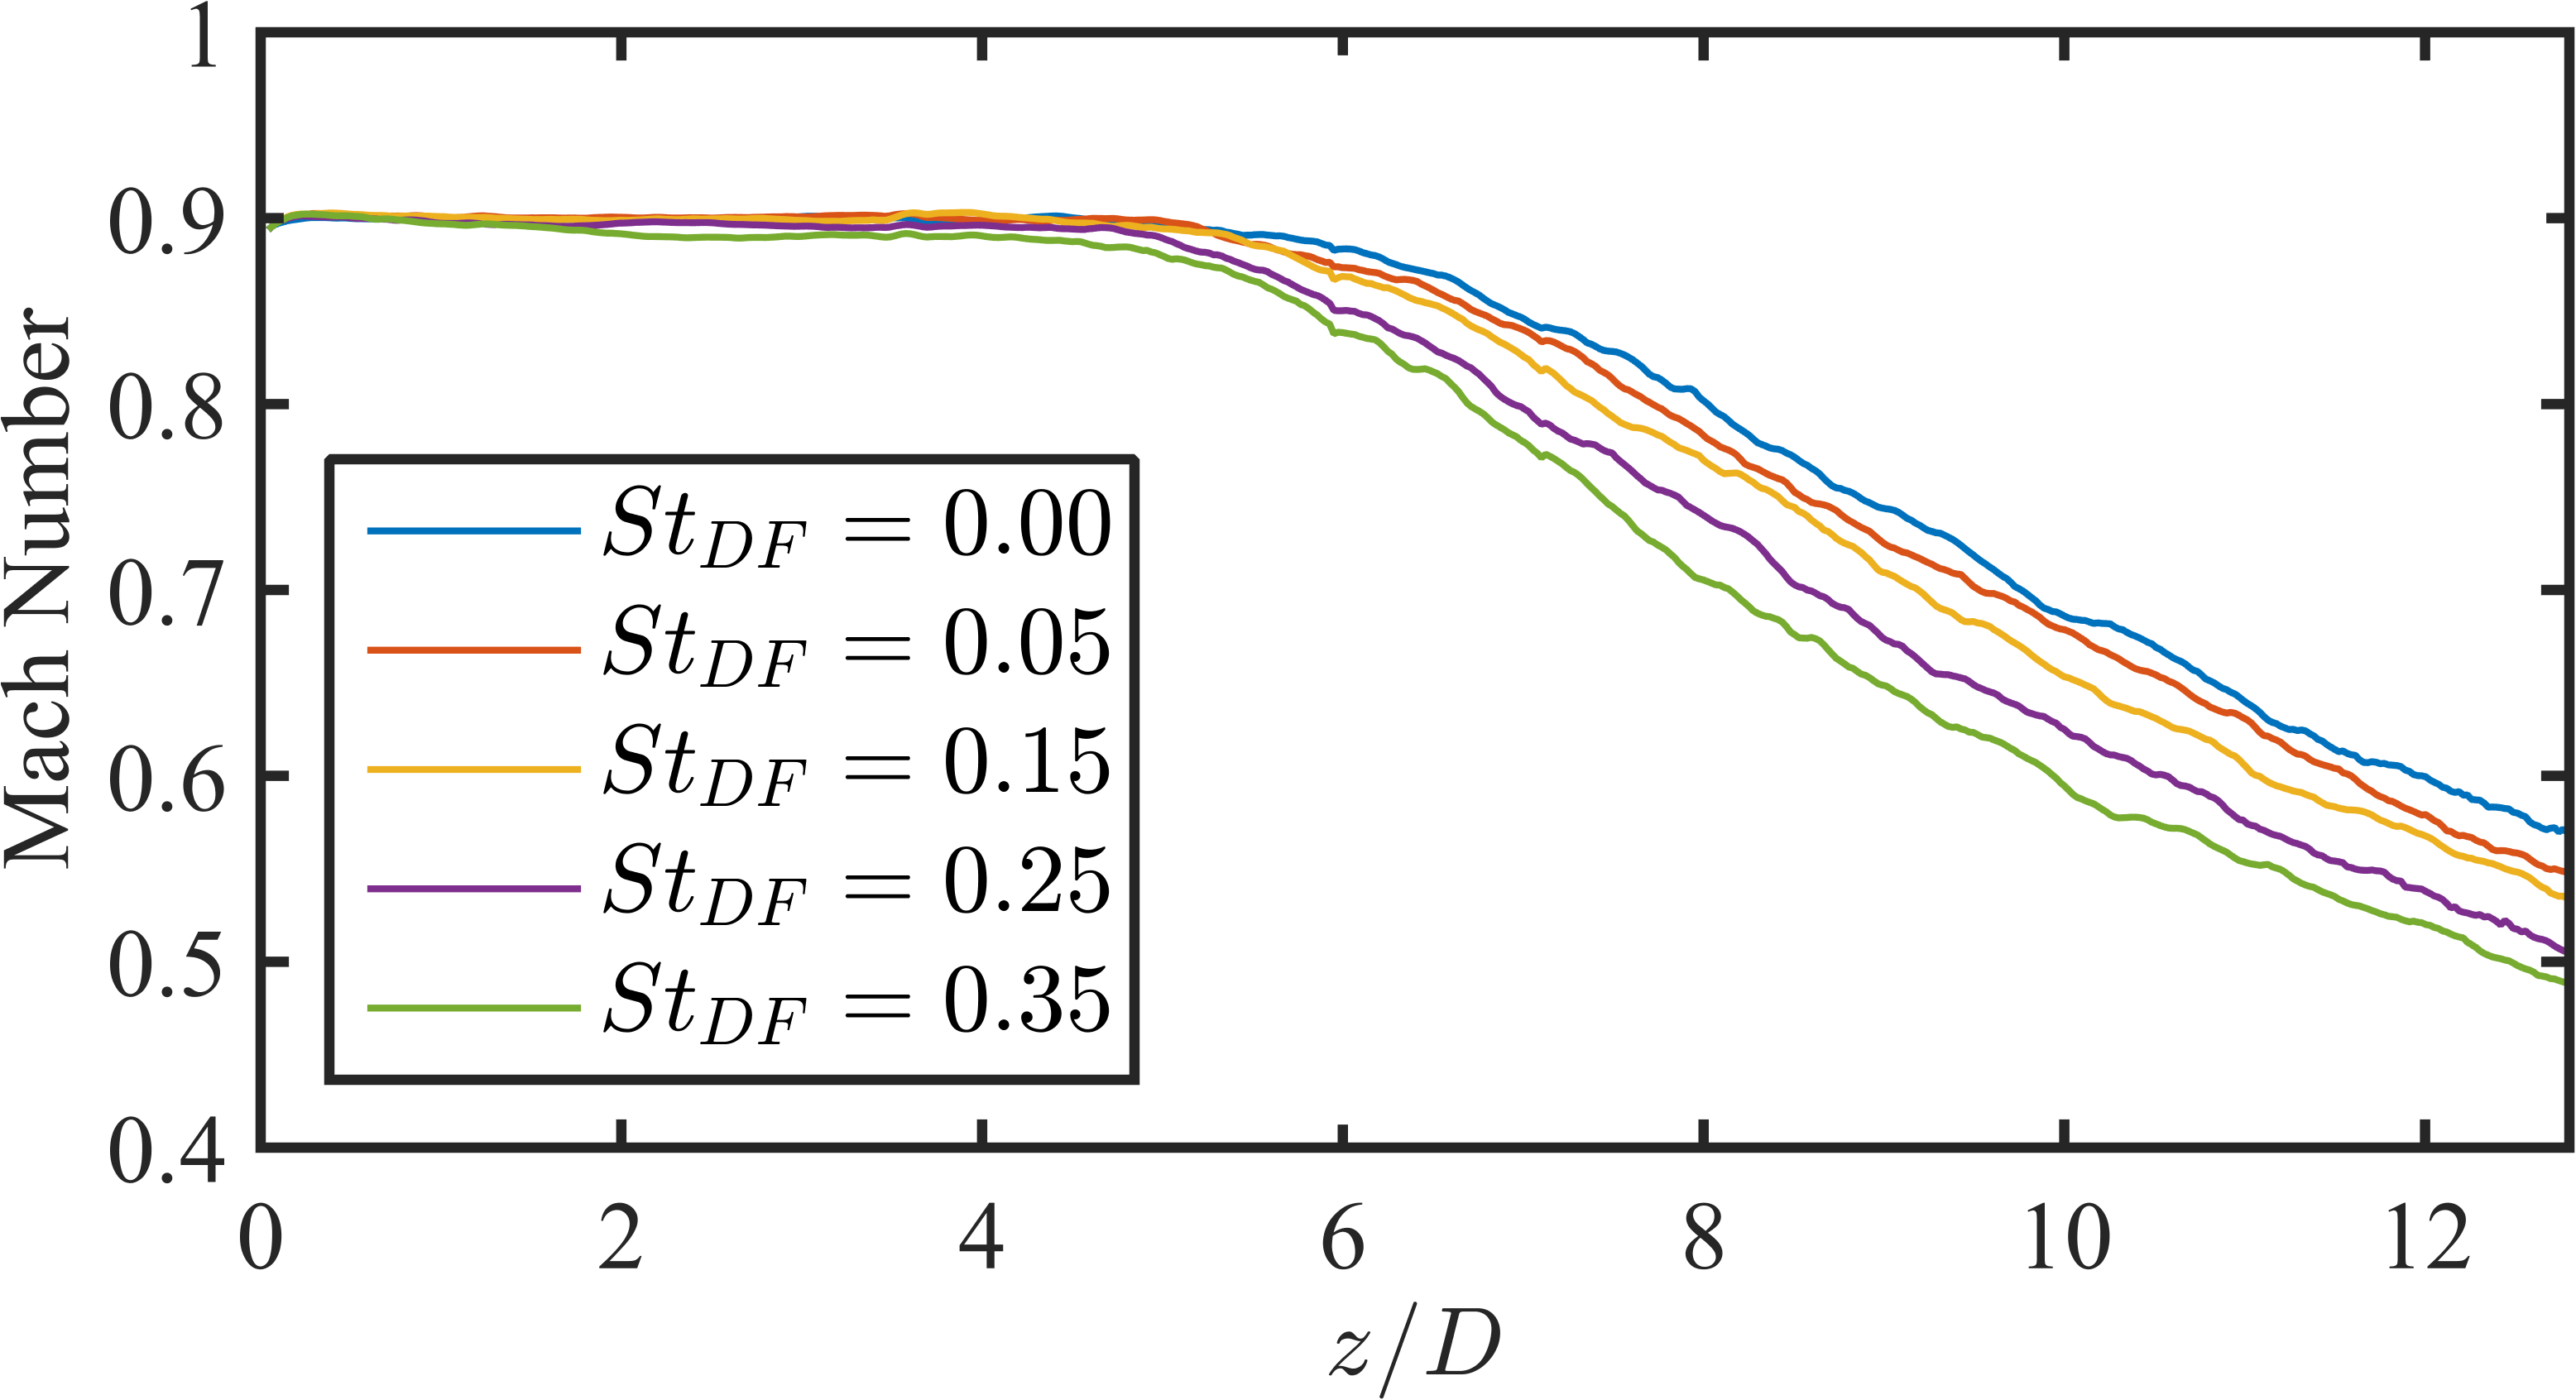
\includegraphics[width = 3.5in]{Figures/ch4_centerlineMach.png}
	\caption{Centerline Mach number for all excitation cases; baseline jet is indicated by `0.00'.}
	\label{fig:ch4_centerlinemach}
\end{figure}


\subsection{Coherent Structure Merging}
In the simulated subsonic shear layer of Wei \& Freund \citep{Wei2006}, optimized control for noise mitigation using generalized actuation was implemented using the adjoint perturbation method.
The methodology was able to ???


\subsection{Large-Scale Structure Disintegration}
Hileman \etal \citep{Hileman2005} investigated the evolution and interactions of large-scale structures and ultimately how these relate to the noise generation process in a supersonic, ideally-expanded jet by combining time-resolved flow visualizations with a three-dimensional microphone array.
Their results showed that the dominant noise was being generated near the end of the potential core, in the region where the shear layers merged.
Large-amplitude, highly-intermittent acoustic events were found to be associated with a fluctuation in the length of the potential core, which the authors ultimately speculated was related to the passage and finally the rapid disintegration of large-scale coherent structures just downstream of the end of the potential core.
The results of \sect{sect:nearfield} also indicated that the jet core region was responsible for the dominant acoustic generation in a subsonic jet, at least to low angles with respect to the jet axis.
The dynamics of the large-scale structures in this region, namely the structure decay, are therefore of particular concern to the current work.

Vortex identification was performed by computing the swirling strength at each instance in the estimated velocity field; details and justification for this method can be found in Adrian \etal \citep{Adrian2000}.
The evolution of the impulsively excited ($St_{DF} = 0.05$) vortex ring has be tracked in \fig{fig:ch4_impulse_structure_disintegration}.
For ease of visualization, a two-dimensional, five-point boxcar filter was applied to the estimated velocity fields prior to computing the swirling strength, and the results have been phase-averaged based on the recorded LAFPA trigger signal.
Lastly, a solid red line has been overlain to approximately match the convective velocity of the structures.
Only a select number of phases are shown here, as a significant amount of dead time between excitations occurs due to the mismatch in the spatial and temporal characteristic frequencies of the large-scale structures.
\begin{figure}
	\centering
	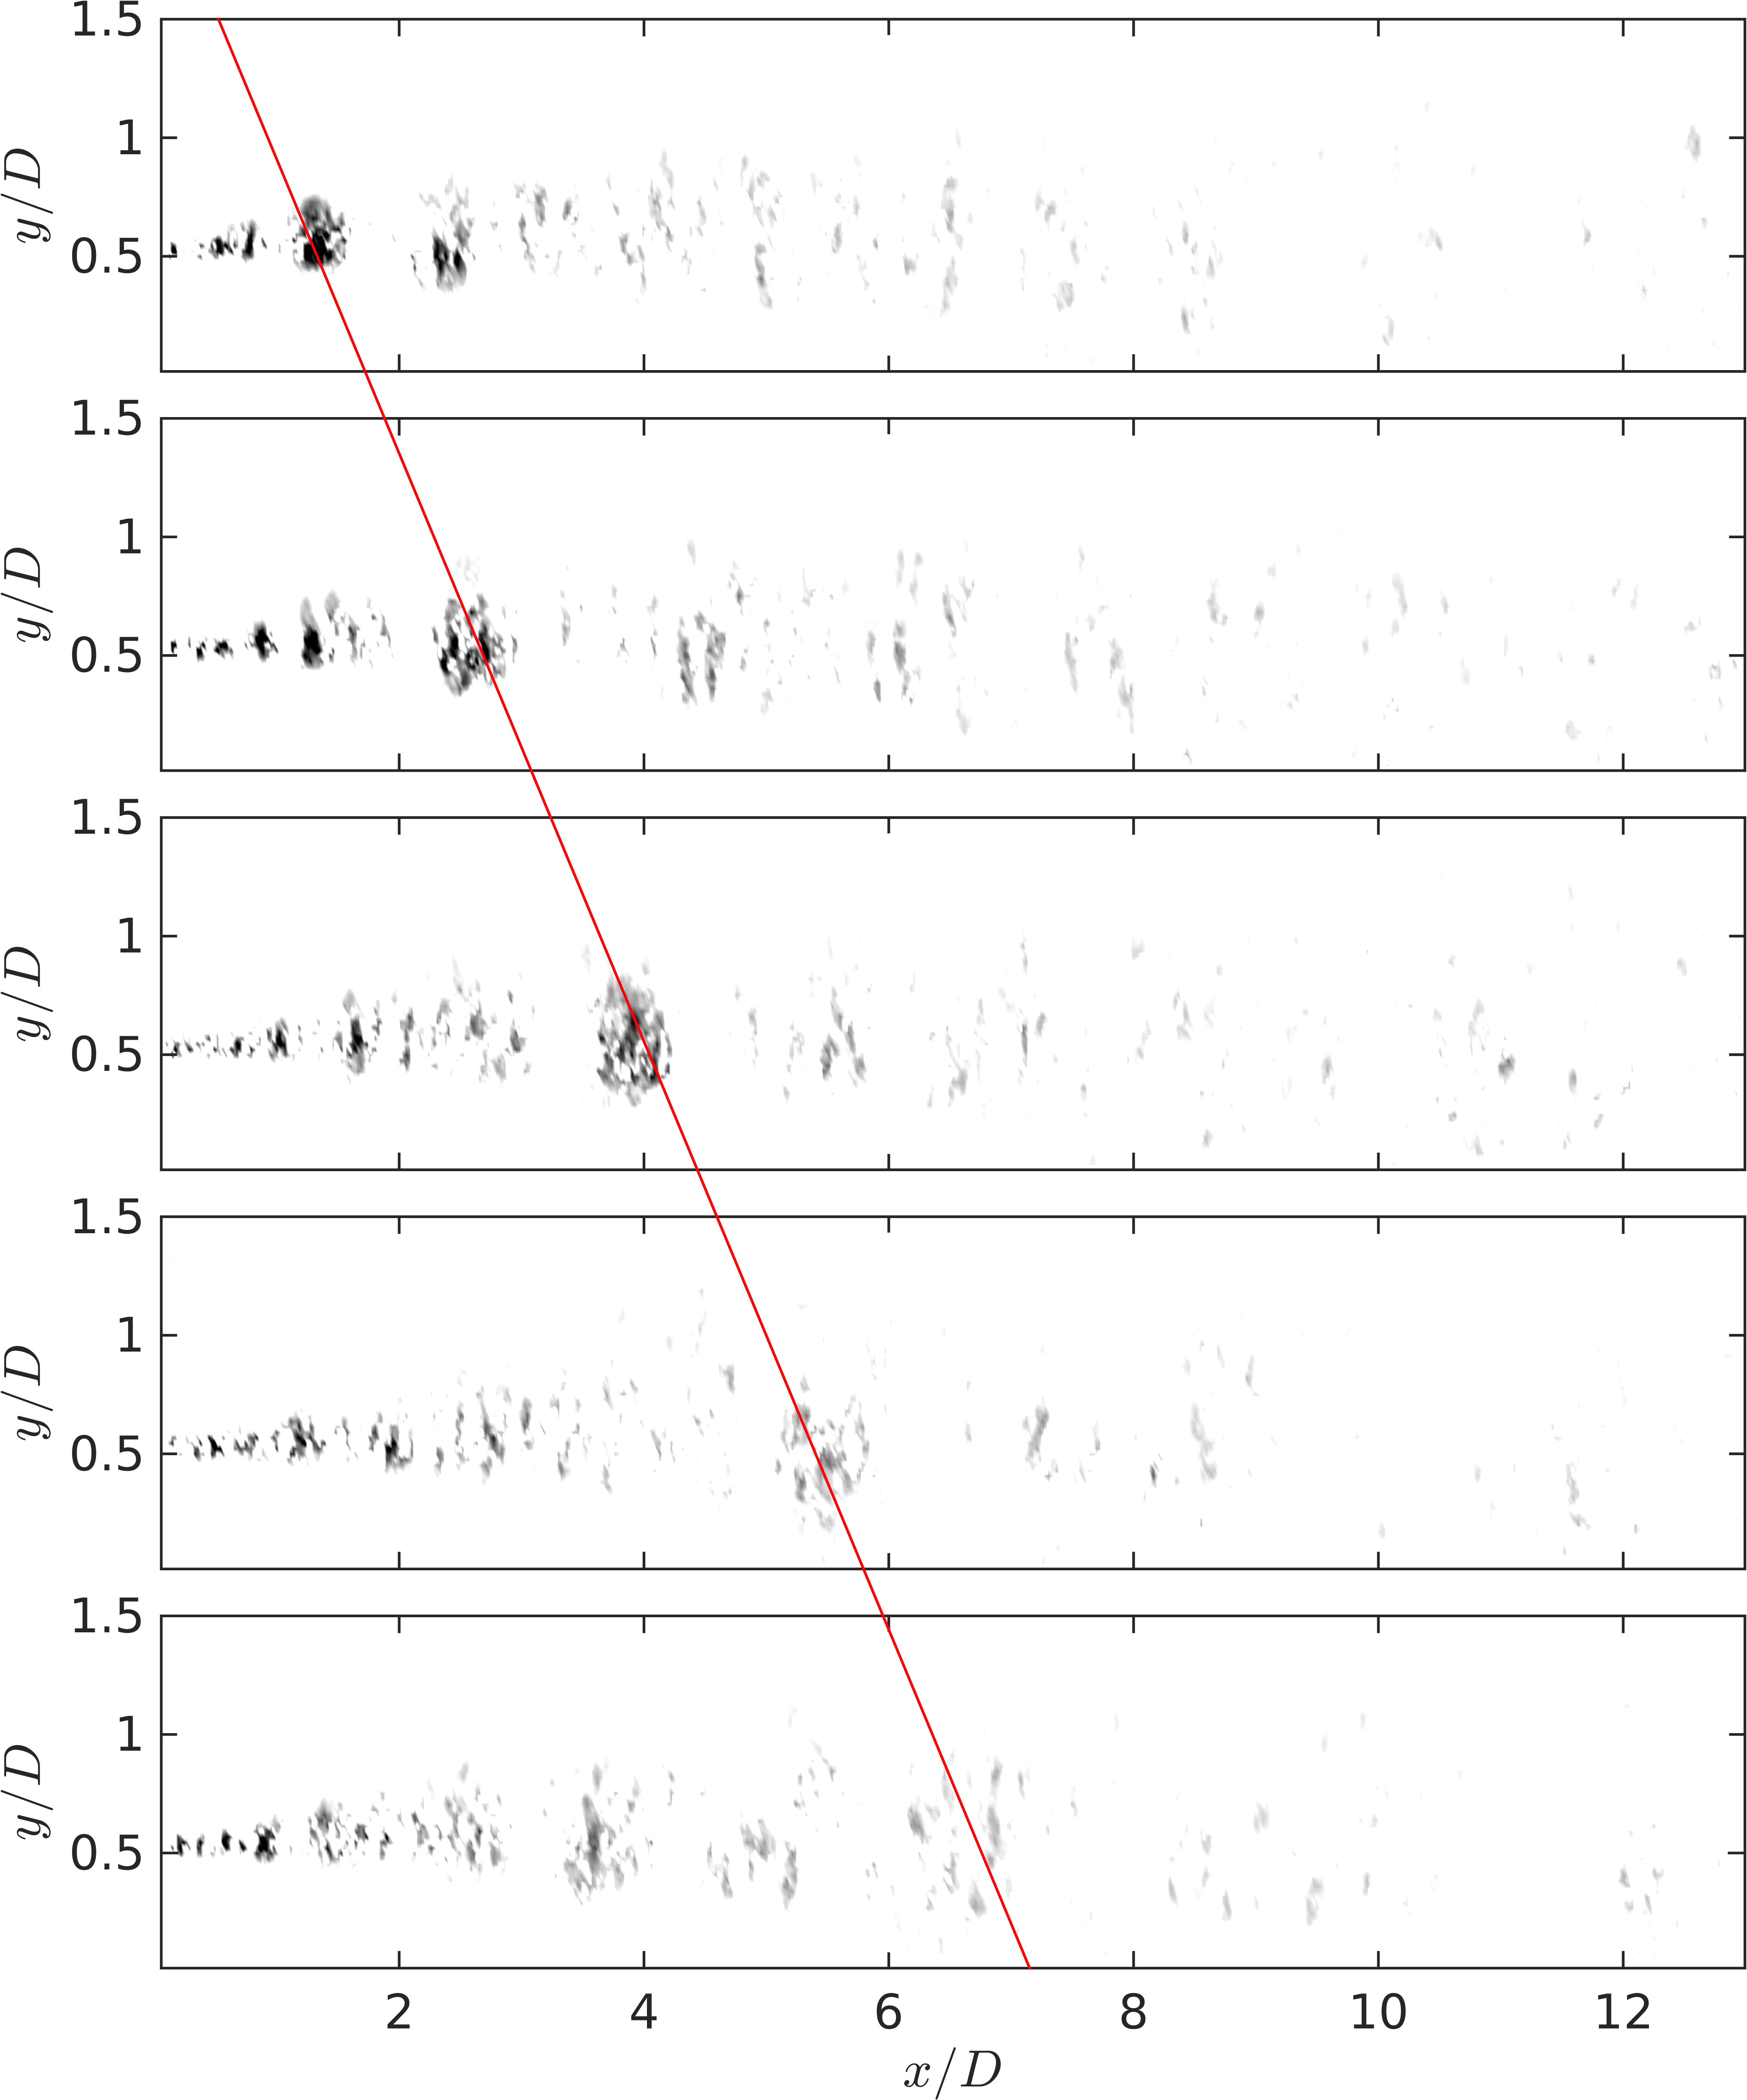
\includegraphics[width=5in]{Figures/ch4_St005_lambda_evolution.png}
	\caption{Evolution of the independent vortex ring ($St_{DF}=0.05$), as visualized using swirling strength. Images are shown at phase steps of roughly $\pi/4$, starting with a phase of $2\pi/3$.}
	\label{fig:ch4_impulse_structure_disintegration}
\end{figure}
As already known from prior experiments at the GDTL \citep{Kearney-Fischer2009}, the excitation produces a strong roll-up of vortical (toroidal) fluid in the near-nozzle region; in the present case the large-scale structure generated by the excitation is clearly discernible over the background turbulence (and experimental/computational noise) by $x/D \simeq 1$.
If the contours of the swirling strength field are to be believed, the rapid growth of the vortex slows by $x/D \simeq 1.5$ and it advects downstream relatively unchanged until  $x/D \simeq 4$ (other vortex identification methods, such as Q-criterion or $\lambda_2$-criterion, were also investigated and a general agreement was found, though swirling strength produced the visually-simplest fields).
\begin{figure}
	\centering
	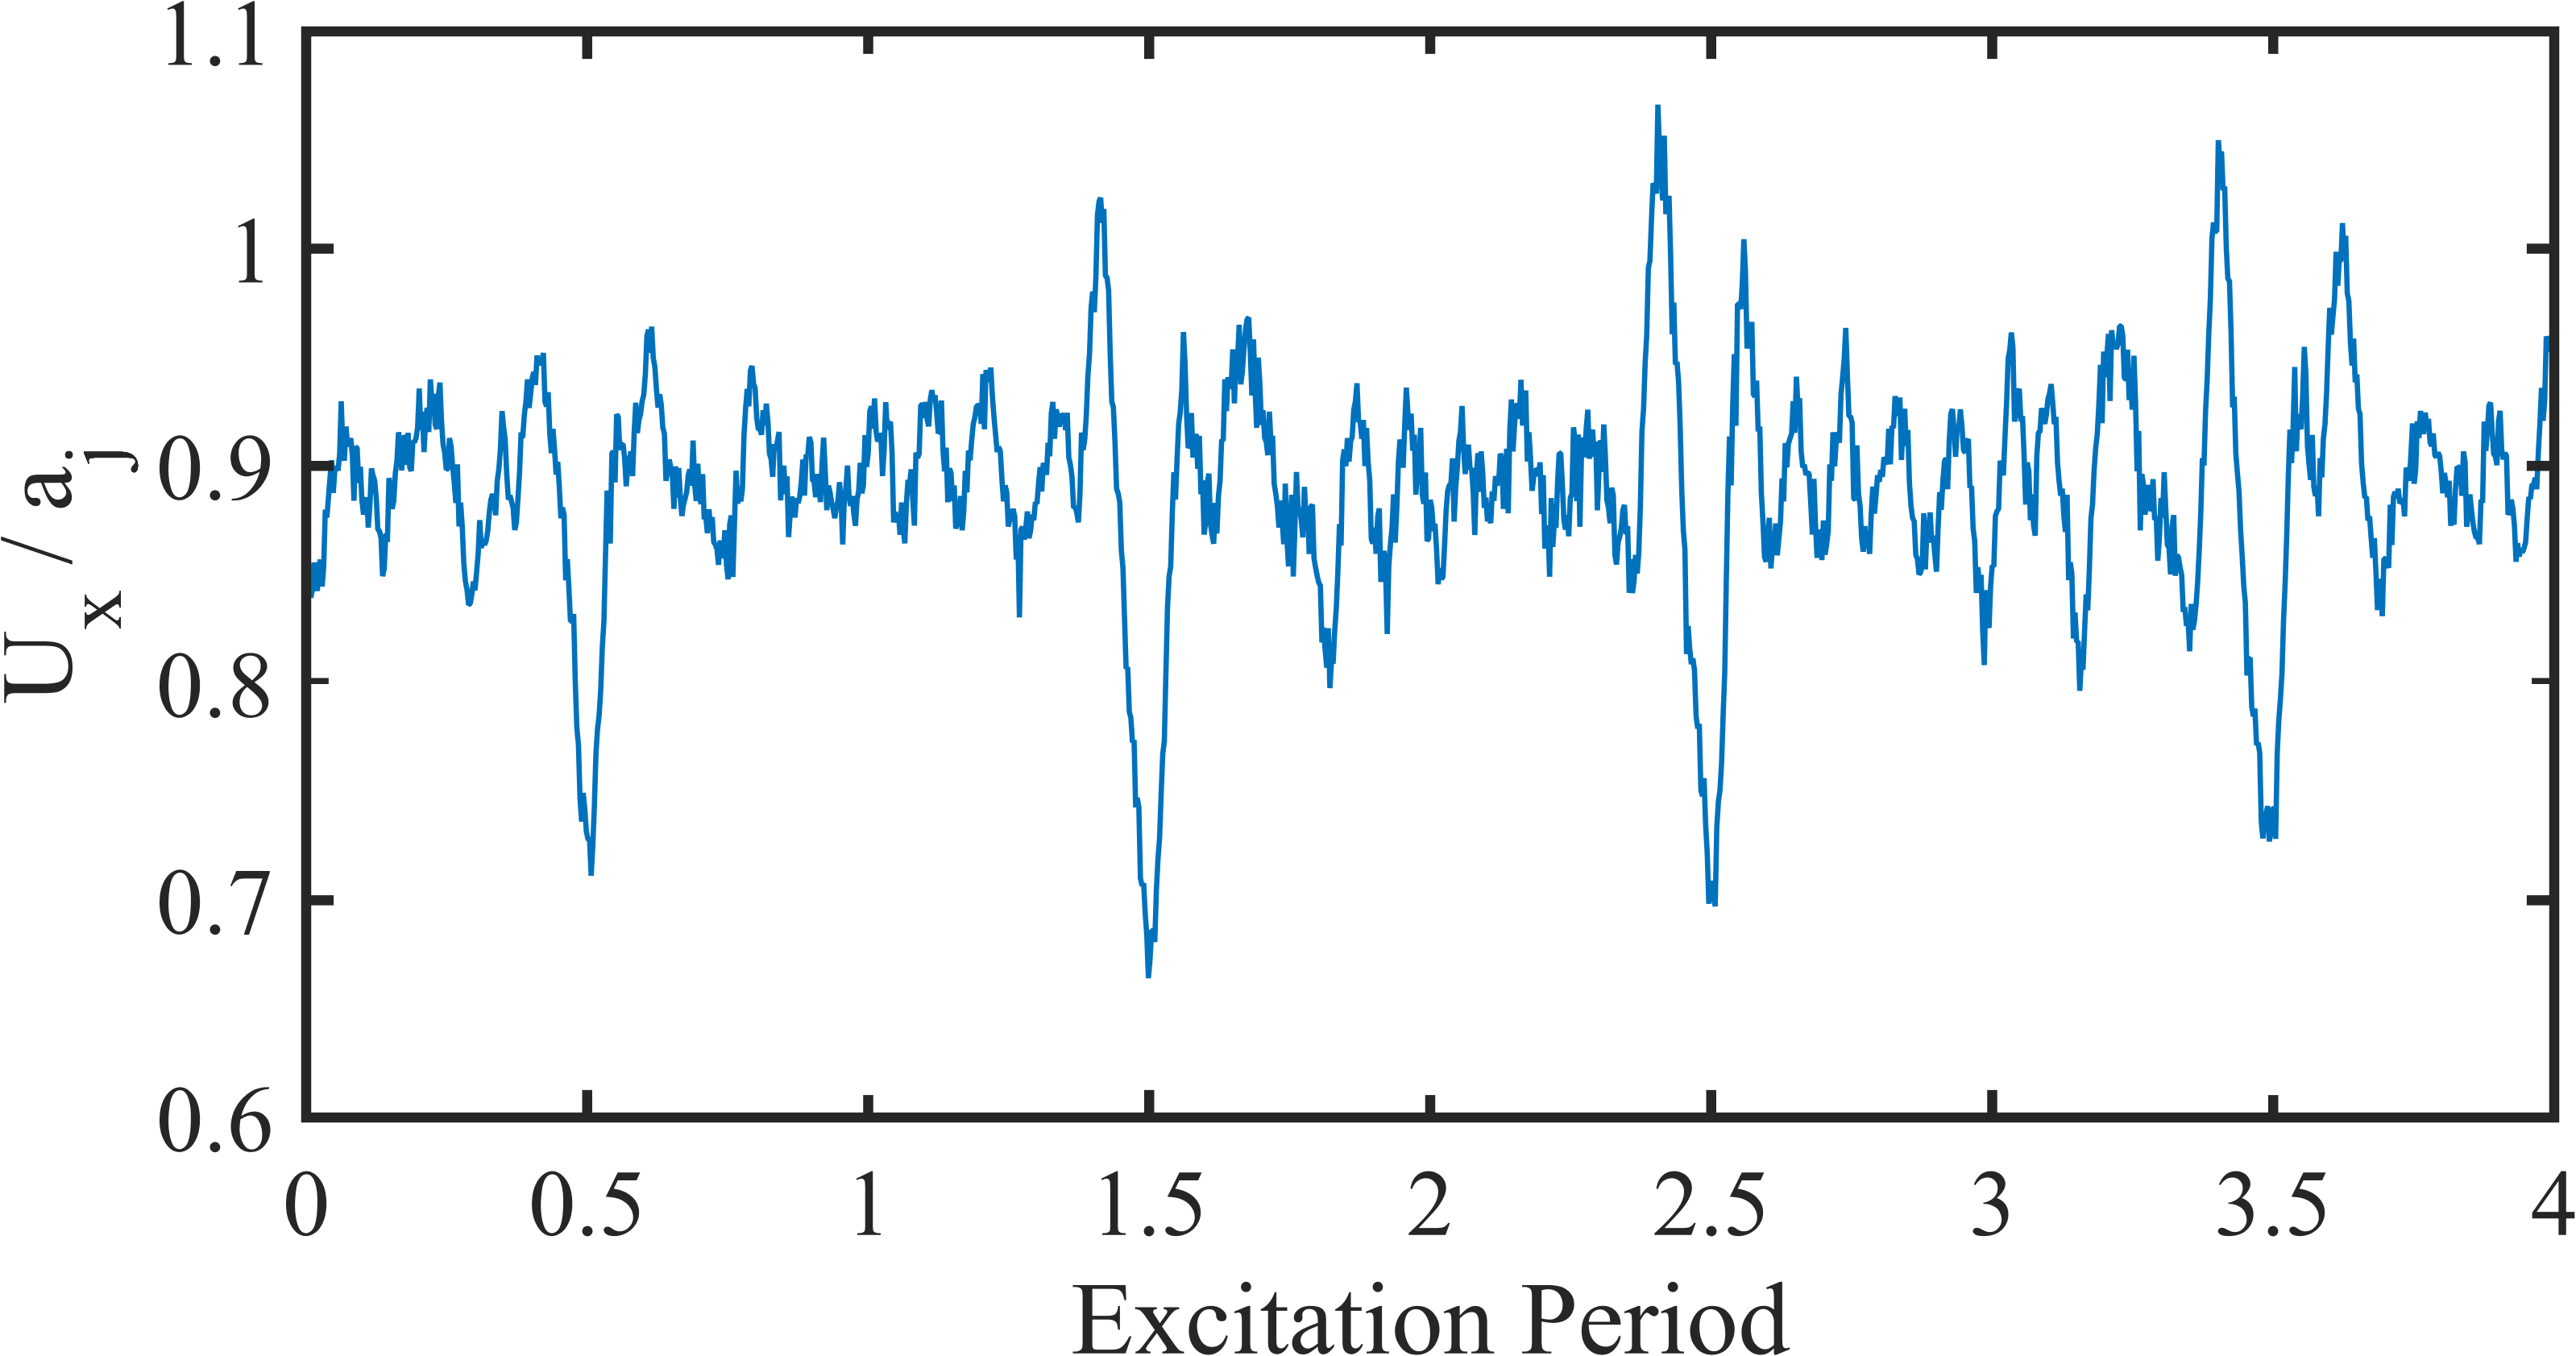
\includegraphics[width=3.5in]{Figures/ch4_St005_centerline_mach_temporal.png}
	\caption{Fluctuations associated with the passage of large-scale structures in the axial velocity along the jet centerline.}
	\label{fig:ch4_St005_centerlinemach_temporal}
\end{figure}